%
% Bachelor / Masterarbeit mit LaTeX
% ===========================================================================
% This is part of the book "Diplomarbeit mit LaTeX".
% Copyright (c) 2002, 2003, 2005, 2007, 2008 Tobias Erbsland
% Copyright (c) 2005, 2006 Andreas Nitsch
% See the file main.tex for copying conditions.
%
% A. DOKUMENTKLASSE
% --------------------------------------------------------------------------

%  1. Definieren der Dokumentklasse.
%     Wir verwenden die KOMA-Script Klasse 'scrbook' für ein Buch.
%
\documentclass[%
    pdftex,%              PDFTex verwenden da wir ausschliesslich ein PDF erzeugen.
    a4paper,%             Wir verwenden A4 Papier.
    twoside,%             zweiseitiger Druck.
 %  openright,
 %  cleardoubleempty,
 %  BCOR12mm,
    12pt,%                Grosse Schrift, besser geeignet für A4.
    parskip=half,%         Halbe Zeile Abstand zwischen Absätzen.
    %chapterprefix,%       Kapitel mit 'Kapitel' anschreiben.
    headsepline,%         Linie nach Kopfzeile.
    %footsepline,%         Linie vor Fusszeile.
    bibliography=totoc,%  
    listof=totoc,%  Literaturverzeichnis im Inhaltsverzeichnis nummeriert einfügen.
    index=totoc%             Index ins Inhaltsverzeichnis einfügen.
]
{scrreprt}

\usepackage[a4paper,% wird eigentlich schon von der Klasse vorgegeben
  head=50mm,headsep=12mm,height=212mm,bottom=45mm]{geometry}

%\setlength{\textwidth}     {15.9cm}    % Textbreite
%\setlength{\oddsidemargin} {0cm}  % linker Rand (2.45-2.54) doppelseitig
%\setlength{\evensidemargin}{0cm}
%\setlength{\paperwidth}    {21.1cm}  % physikalische Seitenbreite
%\setlength{\textheight}    {23.5cm}  % Gesamthöhe für den Seitentext
%\setlength{\topmargin}     {-1cm}    % oberer Rand bis Oberkante Kopfzeile (1.5-2.54)

%
%  2. Festlegen der Zeichencodierung des Dokuments und des Zeichensatzes.
%     Wir verwenden 'UTF-8' für das Dokument,
%     und die 'T1' Codierung für die Schrift.
%
\usepackage[utf8]{inputenc}
\usepackage[T1]{fontenc}

%\usepackage{subfig}
\usepackage{caption}
\usepackage{subcaption}
\usepackage{placeins} 

%
%  3. Packet für die Index-Erstellung laden.
%
\usepackage{makeidx}

%
%  4. Paket für die Lokalisierung ins Deutsche laden.
%     Wir verwenden neue deutsche Rechtschreibung mit 'ngerman'.
%
\usepackage[english]{babel}


%
%  5. Paket für Anführungszeichen laden.
%     Wir setzen den Stil auf 'swiss', und verwenden so die Schweizer
%  Anführungszeichen.
%
\usepackage[style=swiss]{csquotes}


%
%  6. Paket für erweiterte Tabelleneigenschaften.
%
\usepackage{array}
\usepackage{bbm}

%
%  7. Paket um Grafiken im Dokument einbetten zu können.
%     Im PDF sind GIF, PNG, und PDF Grafiken möglich.
%
\usepackage{graphicx}
%
%  8. Pakete für mathematischen Textsatz.
%
\usepackage{amsmath}
\usepackage{amssymb}
\usepackage{dsfont}
\usepackage{mathtools}
%\usepackage{sty/algo}

%
%  9. Paket um Textteile drehen zu können.
%
\usepackage{rotating}

%
% 10. Paket für Farben an verschieden Stellen.
%     Wir definieren zusätzliche benannte Farben.
%
\usepackage{color}

%\usepackage[Lenny]{sty/fncychapleo}
%\usepackage[Glen]{sty/fncychapleo}


%
% 11. Paket für spezielle PDF features.
%
\usepackage[%
    pdftitle={Masterarbeit},%                        Titel des PDF Dokuments.
    pdfauthor={Max Mustermann},%              Autor des PDF Dokuments.
    pdfsubject={Titel der Masterarbeit/Bachelorarbeit},%                    Thema des PDF Dokuments.
    pdfcreator={MiKTeX, LaTeX with hyperref and KOMA-Script},% Erzeuger des PDF Dokuments.
    pdfkeywords={Masterarbeit,Bachelorarbeit,IES},%          Schlüsselwörter für das PDF.(Diese werden von Suchmaschinen auch für PDF Dokumente indexiert.)
    pdfpagemode=UseOutlines,%                                  Inhaltsverzeichnis anzeigen beim Öffnen
    pdfdisplaydoctitle=true,%                                  Dokumenttitel statt Dateiname anzeigen.
    pdflang=de,%  Sprache des Dokuments.
    pdfborder={0 0 0},
]{hyperref}


%
% 12. Paket um Quellcode sauber zu formatieren.
%     Mit der option 'savemem' verschieben wir das laden von
%     einzelnen Programmiersprachen auf einen späteren Zeitpunkt.
%
\usepackage[savemem]{listings}

%
% 13a. Privates Paket für die Schriftart 'Goudy Sans' laden.
%      Dieses Paket ist nur für die publizierte Version des Dokuments gedacht
%      und an dieser Stelle mit den nachfolgenden Anweisungen auskommentiert.
%
%\usepackage{goudysans}

%
% 13a. Font 'Latin Modern Family' verwenden.
%      Verwende dieses Paket wenn du DML selbst kompilierst.
%
\usepackage{lmodern}

%\usepackage{tocbasic}

%
% 15. Für Eingeben von Pseudocode
%

\usepackage[german,ruled,vlined]{algorithm2e}
\usepackage{algorithmic}
\usepackage{multirow}
\usepackage{tabularx,calc}

\usepackage{array} 
% B. EINSTELLUNGEN

% ---------------------------------------------------------------------------
%
%  1. Definieren von eigenen benannten Farben.
%     Für spätere Verwendung in dem Dokument, definieren wir einzelne
%     benannte Farben.
%
\definecolor{LinkColor}{rgb}{0,0,0}
\definecolor{CiteColor}{rgb}{0,0,0}
\definecolor{FileColor}{rgb}{0,0,0}
\definecolor{MenuColor}{rgb}{0,0,0}
\definecolor{UrlColor}{rgb}{0,0,0}
\definecolor{ListingBackground}{rgb}{0.85,0.85,0.85}
%
%  2. KOMA-Script Option, Zeilenumbruch bei Bildbeschreibungen.
%
\setcapindent{1em}

%
%  3. Stil der Kopf- und Fusszeilen.
%     Wir aktivieren mit 'headings' laufende Seitentitel.
%
\pagestyle{headings}

%
%  4. Stil der Überschriften auf normale Schrift.
%     Wir verwenden für die Überschriften den selben Font wie für den Text.
%
\setkomafont{sectioning}{\normalfont\bfseries}       % Titel mit Normalschrift
\setkomafont{captionlabel}{\normalfont\bfseries}     % Fette Beschriftungen
\setkomafont{pagehead}{\normalfont\itshape}          % Kursive Seitentitel
\setkomafont{descriptionlabel}{\normalfont\bfseries} % Fette Beschreibungstitel

%
%  5. Farbeinstellungen für die Links im PDF Dokument.
%
\hypersetup{%
    colorlinks=true,%        Aktivieren von farbigen Links im Dokument (keine Rahmen)
    linkcolor=LinkColor,%    Farbe festlegen.
    citecolor=CiteColor,%    Farbe festlegen.
    filecolor=FileColor,%    Farbe festlegen.
    menucolor=MenuColor,%    Farbe festlegen.
    urlcolor=UrlColor,%     Farbe von URL's im Dokument.
    bookmarksnumbered=true%  Überschriftsnummerierung im PDF Inhalt anzeigen.
}
%
%  6. Einstellungen für das 'listings' Paket.
%
\lstloadlanguages{TeX} % TeX sprache laden, notwendig wegen option 'savemem'
\lstset{%
    language=[LaTeX]TeX,     % Sprache des Quellcodes ist TeX
    numbers=left,            % Zelennummern links
    stepnumber=1,            % Jede Zeile nummerieren.
    numbersep=5pt,           % 5pt Abstand zum Quellcode
    numberstyle=\tiny,       % Zeichengrösse 'tiny' für die Nummern.
    breaklines=true,         % Zeilen umbrechen wenn notwendig.
    breakautoindent=true,    % Nach dem Zeilenumbruch Zeile einrücken.
    postbreak=\space,        % Bei Leerzeichen umbrechen.
    tabsize=2,               % Tabulatorgrösse 2
    basicstyle=\ttfamily\footnotesize, % Nichtproportionale Schrift, klein für den Quellcode
    showspaces=false,        % Leerzeichen nicht anzeigen.
    showstringspaces=false,  % Leerzeichen auch in Strings ('') nicht anzeigen.
    extendedchars=true,      % Alle Zeichen vom Latin1 Zeichensatz anzeigen.
    backgroundcolor=\color{ListingBackground}} % Hintergrundfarbe des Quellcodes setzen.

%
% C. NEUE MAKROS UND UMGEBUNGEN
% ---------------------------------------------------------------------------

\setcounter{secnumdepth}{4}
\setcounter{tocdepth}{3}
%
%  1. Umgebung für Änerungsliste mit einem speziellen Aufzählungszeichen.
%
\newenvironment{ListChanges}%
    {\begin{list}{$\diamondsuit$}{}}%
    {\end{list}}

%
%  2. Ersatz für die \LaTeX und \TeX Befehle für korrekte Darstellung.
%     Wir verwenden die 'Latin Modern Family' ('lm') als Font, da diese im
%     vergleich zu 'Computer Modern' ('cm') auch PostScript Dateien
%     anbieten, was zu einer schöneren Darstellung im PDF führt.
%
\newcommand{\DMLLaTeX}{{\fontfamily{lmr}\selectfont\LaTeX}}
\newcommand{\DMLTeX}{{\fontfamily{lmr}\selectfont\TeX}}

\newcommand{\HRule}{\rule{\linewidth}{0.5mm}}

\newcommand\addToPageCenter[1]{%
			\AddToShipoutPicuture*{\AtPageCenter{%
			\makebox(0,0){\includegraphics%
			[width=0.9\paperwidth]{#1}}}}}
			
			%%%% Abkürzungen für Befehle %%%%%
\newcommand{\bi}{\begin{itemize}}
\newcommand{\ei}{\end{itemize}}
\newcommand{\bc}{\begin{center}}
\newcommand{\ec}{\end{center}}
\newcommand{\bt}{\begin{tabular}}
\newcommand{\et}{\end{tabular}}
\newcommand{\ba}{\begin{array}}
\newcommand{\ea}{\end{array}}
\newcommand{\be}{\begin{enumerate}}
\newcommand{\ee}{\end{enumerate}}
\newcommand{\balg}{\begin{algorithm}}
\newcommand{\ealg}{\end{algorithm}}
\newcommand{\abs}[1]{\left\vert#1\right\vert}
\newcommand{\norm}[1]{\left\Vert#1\right\Vert}
\newcommand{\scalarproduct}[2]{\left<#1\vphantom{#2} \right| \! %
                                       \left.\vphantom{#1}#2\right>}
\newcommand{\scp}[2]{\scalarproduct{#1}{#2}}


\def\AmS{$\mathcal{A}$\kern-.1667em\lower.5ex\hbox
    {$\mathcal{M}$}\kern-.125em$\mathcal{S}$}
\def\AmSmath{\AmS{}math}
\usepackage{textcomp} 

\newcommand{\kommentar}[1]{}


%
% D. AKTIONEN
% ---------------------------------------------------------------------------
\newcommand*\restoreclearpage{}
\newcommand*\restorecleardoublepage{}
 \renewcommand*{\partheadendvskip}{%
 %\vfil\newpage
	\vspace{2cm}
  \expandafter\gdef\expandafter\restoreclearpage
  \expandafter{\expandafter\gdef\expandafter\clearpage
  \expandafter{\clearpage}}%
  \expandafter\gdef\expandafter\restorecleardoublepage
  \expandafter{\expandafter\gdef\expandafter\cleardoublepage
  \expandafter{\cleardoublepage}}%
  \gdef\clearpage{\restoreclearpage\restorecleardoublepage}%
  \global\let\cleardoublepage\clearpage
}

\newcommand{\changefont}[3]{
\fontfamily{#1} \fontseries{#2} \fontshape{#3} \selectfont}

\DeclareMathOperator*{\argmin}{argmin}
\DeclareMathOperator*{\argmax}{argmax}
\DeclareMathOperator*{\sign}{sgn}

%  1. Index erzeugen.
%
\makeindex
\pdfminorversion=6
%
% E. SILBENTRENNUNG
% ---------------------------------------------------------------------------
%
% Beispiele für Silbentrennungen

\hyphenation{Sach-bü-cher Mas-ter-ar-beit}

%
% ===========================================================================
% EOF
%
\begin{document}
%
% Diplomarbeit mit LaTeX
% ===========================================================================
% This is part of the book "Diplomarbeit mit LaTeX".
% Copyright (c) 2002-2005,2007 Tobias Erbsland
% Copyright (c) 2005 Andreas Nitsch
% See the file diplomarbeit_mit_latex.tex for copying conditions.
%

\begin{titlepage}
    \begin{center}
    

    \vspace*{0.5cm}

    \large{Faculty of Electrical Engeneering and Computer Science}\\
    \vspace*{0.5cm} \large{Department of Intelligent Embedded Systems\\ Prof.
    Dr. rer. nat. Bernhard Sick}

    \vspace*{2cm}
 		% BITTE EINES DER BEIDEN WÄHLEN!! %
    \large {BACHELOR'S THESIS}\\
    \vspace*{1cm} \Huge {\textbf{Time Series Denoising Diffusion Probabilistic Models and Continual Learning} }\\
    \vspace*{1cm}

    \normalsize{written by} \\
    \large{Nikita Popkov} \\
    \vspace*{1.5cm} \normalsize{\today}

    \vspace*{1cm}

        \begin{center}
            \begin{tabular}{ll}
             First Supervisor: & Prof. Dr. rer. nat. Bernhard Sick\\
             Second Supervisor: & Prof. Dr.-Ing. Christian A. Hans \\
            \end{tabular}
        \end{center}

    \end{center}
\end{titlepage}
\cleardoublepage
\pagenumbering{roman}
\chapter*{Abstract}

% Aktuelle Seitenzahl in einem Zähler speichern
% -> römische Seitennummerierung soll durchgängig
% sein und wird nachher wieder aufgegriffen.

\newcounter{zusammen_seitenzahl}
\setcounter{zusammen_seitenzahl}{\value{page}}

%\addcontentsline{toc}{chapter}{Zusammenfassung}
This thesis focuses on exploring Denoising Diffusion Probabilistic Models (DDPM) in respect to time series data distributions. 
Knowledge about image generating DDPMs is used to create Time Series DDPMs that are capable of synthesizing time series data. Different statistical, visual metrics as well as an applicative test are introduced to evaluate the quality of the generative models. In conducting this applicative test, not only is the quality of the models further measured, but also the investigation is carried out to determine whether a trained DDPM can perform in a continual learning environment.

\tableofcontents
\cleardoublepage
\pagenumbering{arabic}
\chapter{Introduction}
\label{sec:introduction}
\section{Motivation}
\label{sec:motivation}
A need for synthetic data distributions is on the rise and the trend doesn't seem to slow down. 
The last years held great advantages in the field of generative models, especially in the domain of image generation.
Big institutions like OpenAI, StabilityAI or others provided the necessary velocity that drove mayor improvements. Starting out with rather
poor results the models were capable of learning basic contexts of images but the overall quality was bad. In the following years a new architecture
emerged \cite{ho_denoising_2020} \cite{nichol_improved_2021} and soon outperformed the former best performing models \cite{dhariwal_diffusion_2021}. 
Those rapid improvements led to a high velocity research environment regarding this topic. Commercial and open-source applications like DALLE or Stable Diffiusion emerged.
As seen in fig. \ref{fig:sd images} open source models like Stable Diffusion empower people to generate their own images locally on their home computer.
These applications mostly relied on Denoising Diffusion Probabilistic Models (DDPM). After achieving such great results in the domain of image generation, the decision was made to apply those models to another domain of data - specifically, time series data. Reworking the DDPM architecture so it can handle time series samples is the main task. This might lead
to a new way of synthesizing time series data. DDPM consist only of one model that is easy to understand and training is a simple process, which give them a practical advantage.
In comparison to one other prominent model type like Generative Adversarial Networks \cite{Goodfellow_2017}, DDPM don't rely on a second model which renders the training significantly less complex.
\begin{figure*}
    \centering
    \begin{subfigure}{0.5\textwidth}
        \centering
        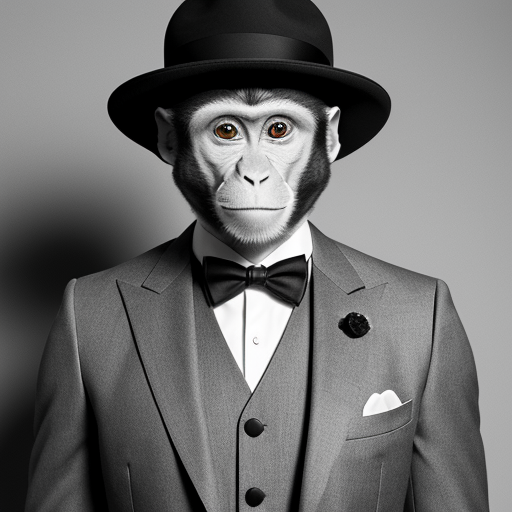
\includegraphics[width=0.5\linewidth]{images/sd1.png}
        \caption[Monkey with tuxedo and hat]%
        {{\small Monkey with tuxedo and hat}}    
        \label{fig:sd1}
    \end{subfigure}%
    \begin{subfigure}{0.5\textwidth}  
        \centering 
        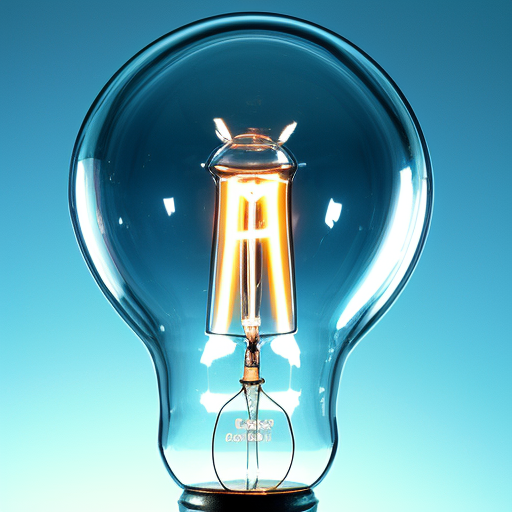
\includegraphics[width=0.5\linewidth]{images/sd2.png}
        \caption[Light bulb]%
        {{\small Light bulb}}    
        \label{fig:sd2}
    \end{subfigure}\\
    \begin{subfigure}{0.5\linewidth}   
        \centering 
        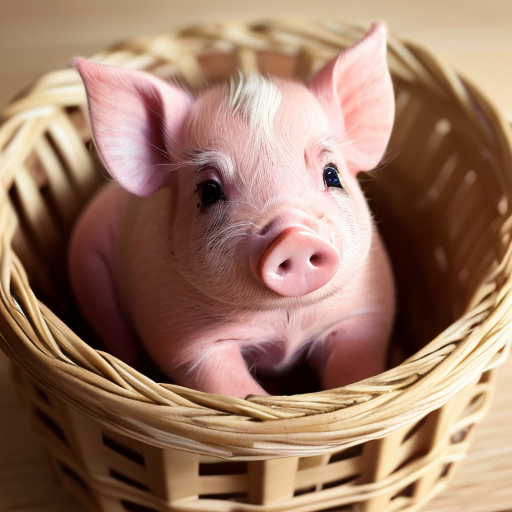
\includegraphics[width=0.5\linewidth]{images/sd3.png}
        \caption[Pig in a basket]%
        {{\small Pig in a basket}}    
        \label{fig:sd3}
    \end{subfigure}%
    \begin{subfigure}{0.5\linewidth}   
        \centering 
        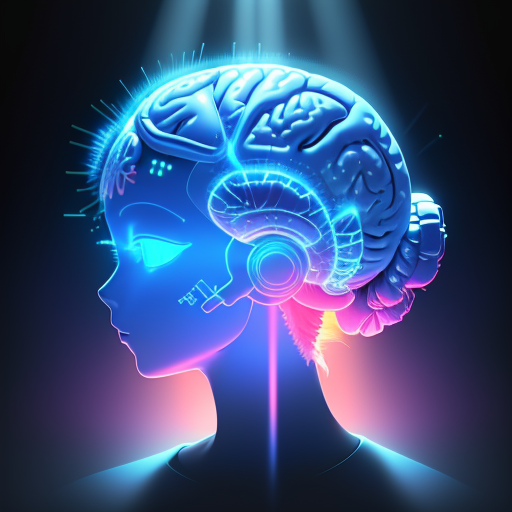
\includegraphics[width=0.5\linewidth]{images/sd4.png}
        \caption[Artistic depiction of an AI]%
        {{\small Artistic depiction of an AI}}    
        \label{fig:sd4}
    \end{subfigure}%
    \caption[ Locally generated images using Stable Diffusion 1.5 ]
    {\small Locally generated images using Stable Diffusion 1.5.} 
    \label{fig:sd images}
\end{figure*}

\section{Contribution}
\label{sec:contribution}

The contribution of this thesis is to investigate whether DDPM are considerable models for the task of 
time series synthesis. Representing the information context of a certain time series distribution can have a supportive
role for different anonymization tasks, forecasting task and data pipelines. For this purpose, the DDPM architecture was reworked to align with the requirements of working with time series data. Following a set of statistical means is defined to evaluate the generated samples.
As another layer of evaluation an applicative test is introduced. This test consists of using our trained models in continual learning scenario, so this thesis also shines light on the question if 
a trained DDPM can perform in a Continual Learning environment that is based on time series data.

\section{Content Structure}
\label{sec:contentstructure}

This section gives an overview of the contents of each chapter in this thesis.

\textbf{Chapter \ref{sec:introduction} Introduction}

A basic summarization of the contents that are presented in this thesis.

\textbf{Chapter \ref{sec:foundations} Foundations}

An overview and comprehensive explanation of all foundations that are necessary to understand the contents of this thesis.

\textbf{Chapter \ref{sec:stateoftheart} State of the art}

A look into the scientific landscape surrounding the questions that are investigated in this thesis.
Naming different approaches that where considered by others to answer the same or similar questions.

\textbf{Chapter \ref{sec:approach} Approach}

A description of the implemented methods and models. Showing a sketch of the framework that was build.

\textbf{Chapter \ref{sec:datasets} Datasets}

An overview of all datasets that were used for the machine learning tasks. Also details about the structure, size and content of each dataset.

\textbf{Chapter \ref{sec:experiments} Experiments}

A definition of specific experimental environments that are used to guaranty a coherent evaluation of the results gathered during 
the investigations.

\textbf{Chapter \ref{sec:results} Results}

An evaluation and discussion of the results that were found during the experiments.

\textbf{Chapter \ref{sec:application} Applications}

A description of different sectors or fields of research this work can be practically used in. 

\textbf{Chapter \ref{sec:conclusion} Conclusion}

A final conclusion that summarizes all results and answers that where found during the thesis work.




\chapter{Foundations}
\label{sec:foundations}
Firstly, a description of basic but significant architectures that are used in this thesis. Starting by convolutions and then describing more complex architectures like the UNET in section \ref{sec:unet}. Next, the main generative approach explored in this thesis, the Denoising Diffusion Probabilistic Model, will be described. A rough overview of the statistical and visual metrics that were used to evaluate the results in section \ref{sec:results} are given. Finally, discussions about the topic of Continual Learning and how it is defined.
\section{Convolutions}
\label{sec:convolutions}
The principals of Convolutional Neural Networks (CNN) were first described by Fukushima in \cite{Fukushima1980NeocognitronAS}. The name CNN was not set by the time the article was released,
but the idea is used today in many models is still the same. A CNN is a type of neural network designed to process visual or spacial inputs, e.g. images, videos, audio signals or even time series. \newline
A CNN consists of one or more convolutional layers.
A convolutional layer is described as a layer that performs mathematical operations on the input.Those are called convolutions. Convolutions combine the input data with a given set of
filters or kernels, that can be described as specially weighted matrices that are capable of detecting specific features or patterns in the given data. Those features can be edges, corners, different colors, textures or shapes.
This operation is performed by sliding the kernel over the input data and computing the dot product between the kernel and the exposed area of the data as seen in figure \ref{fig:cnn dot}
\begin{figure}
    \centering
    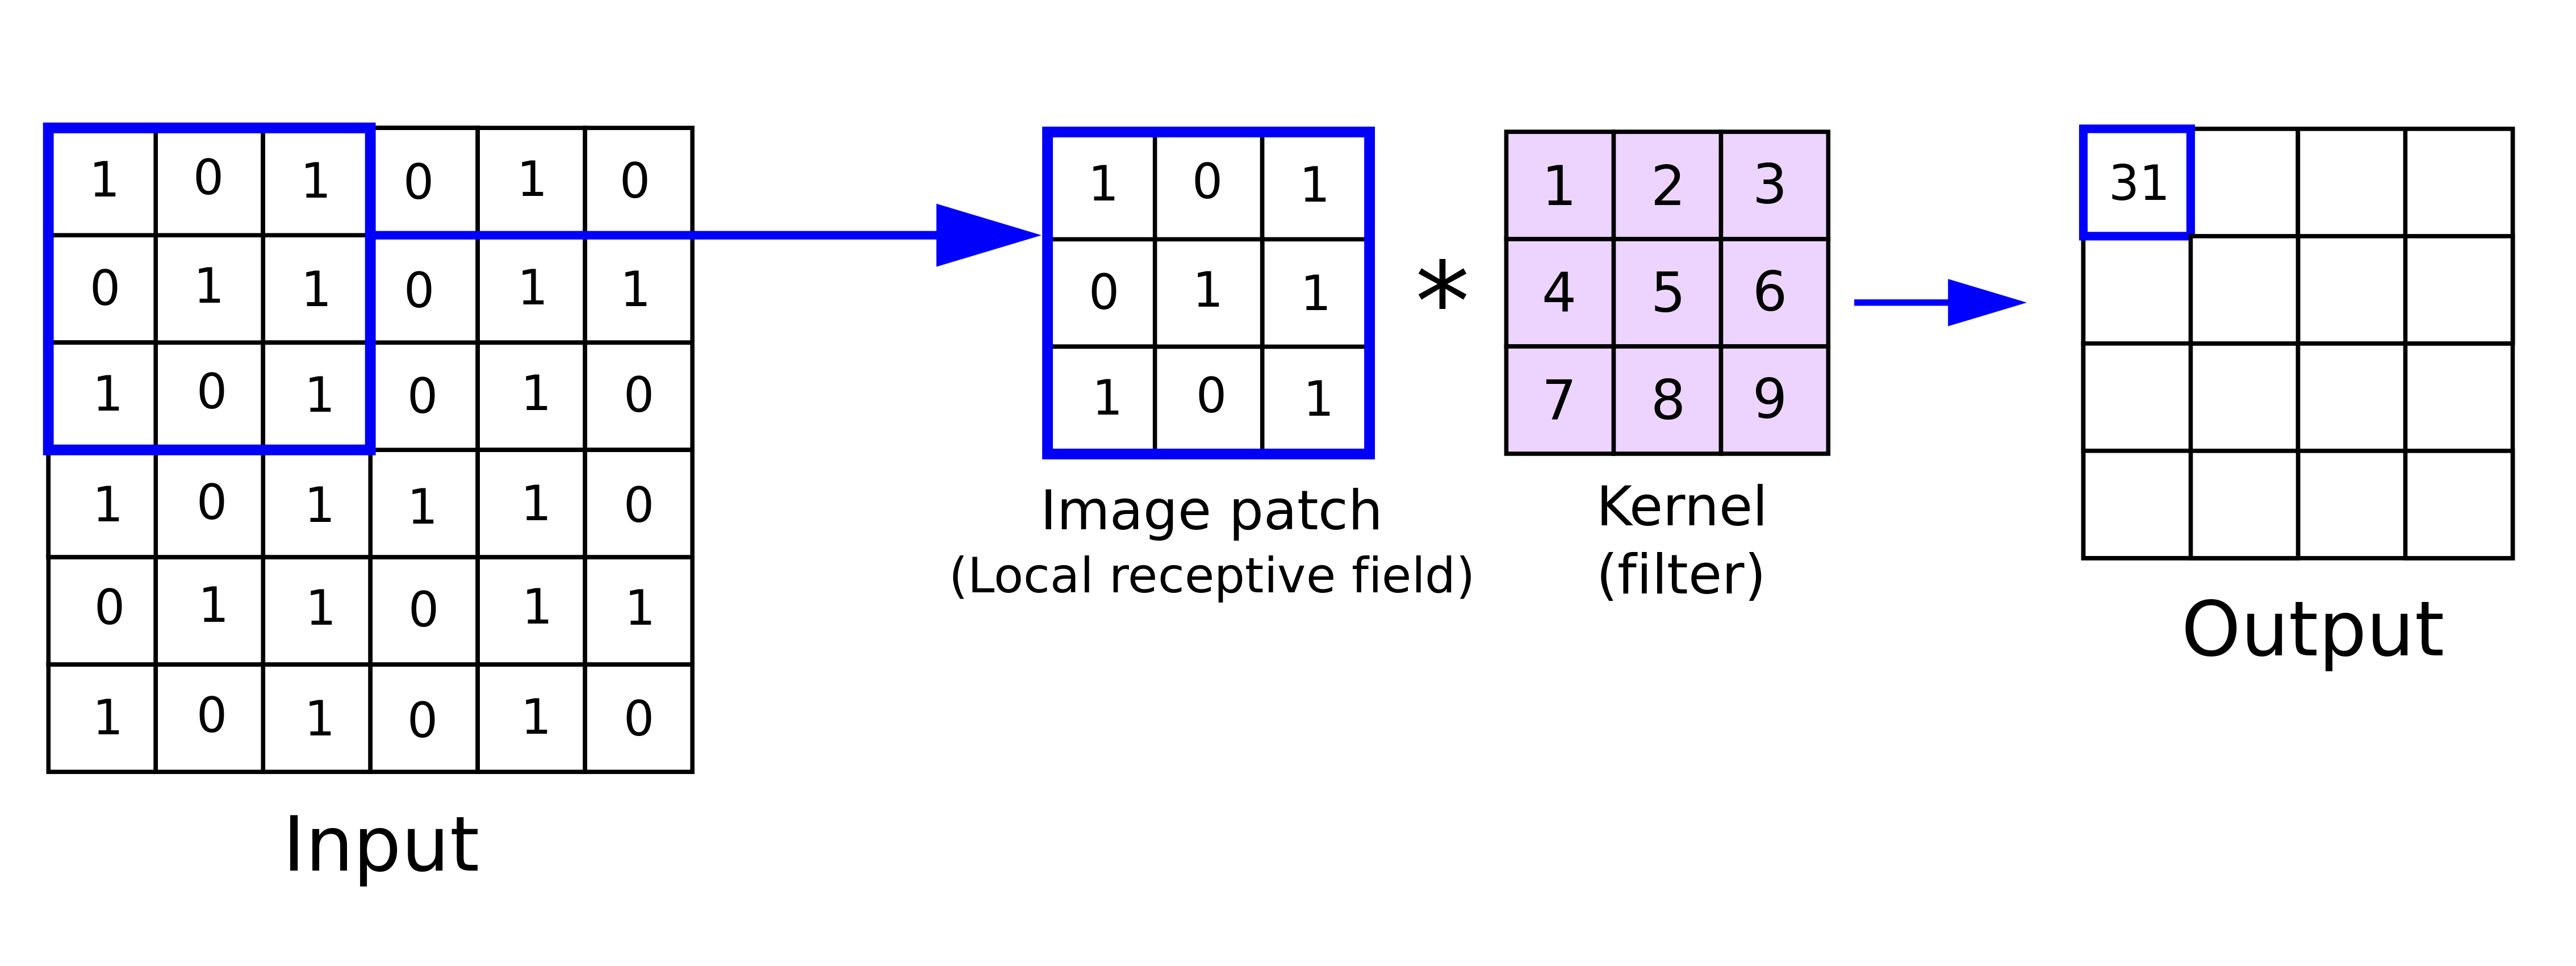
\includegraphics[width=0.85\textwidth]{images/cnn-dot.png}
    \caption{A visualization of a convolutional operation}
    \label{fig:cnn dot}
\end{figure}
\section{UNET}
\label{sec:unet}
The UNET was introduced to tackle the task of image segmentation \cite{ronneberger_unet}. Not an easy task to solve, as it requires 
both high-level semantic information and low-level spatial information of the image.
Traditional convolutional neural networks are good at extracting semantic features, but they tend to lose spatial information due to pooling 
and striding operations that reduce the resolution of the feature maps.
To address this issue, a powerful deep learning architecture called UNET was proposed by Ronneberger et al. in 2015 . 
UNET is based on the idea of Fully Convolutional Networks (FCN), which use only convolutional layers to perform end-to-end 
image segmentation without any fully connected layers. \newline
\begin{figure}
    \centering
    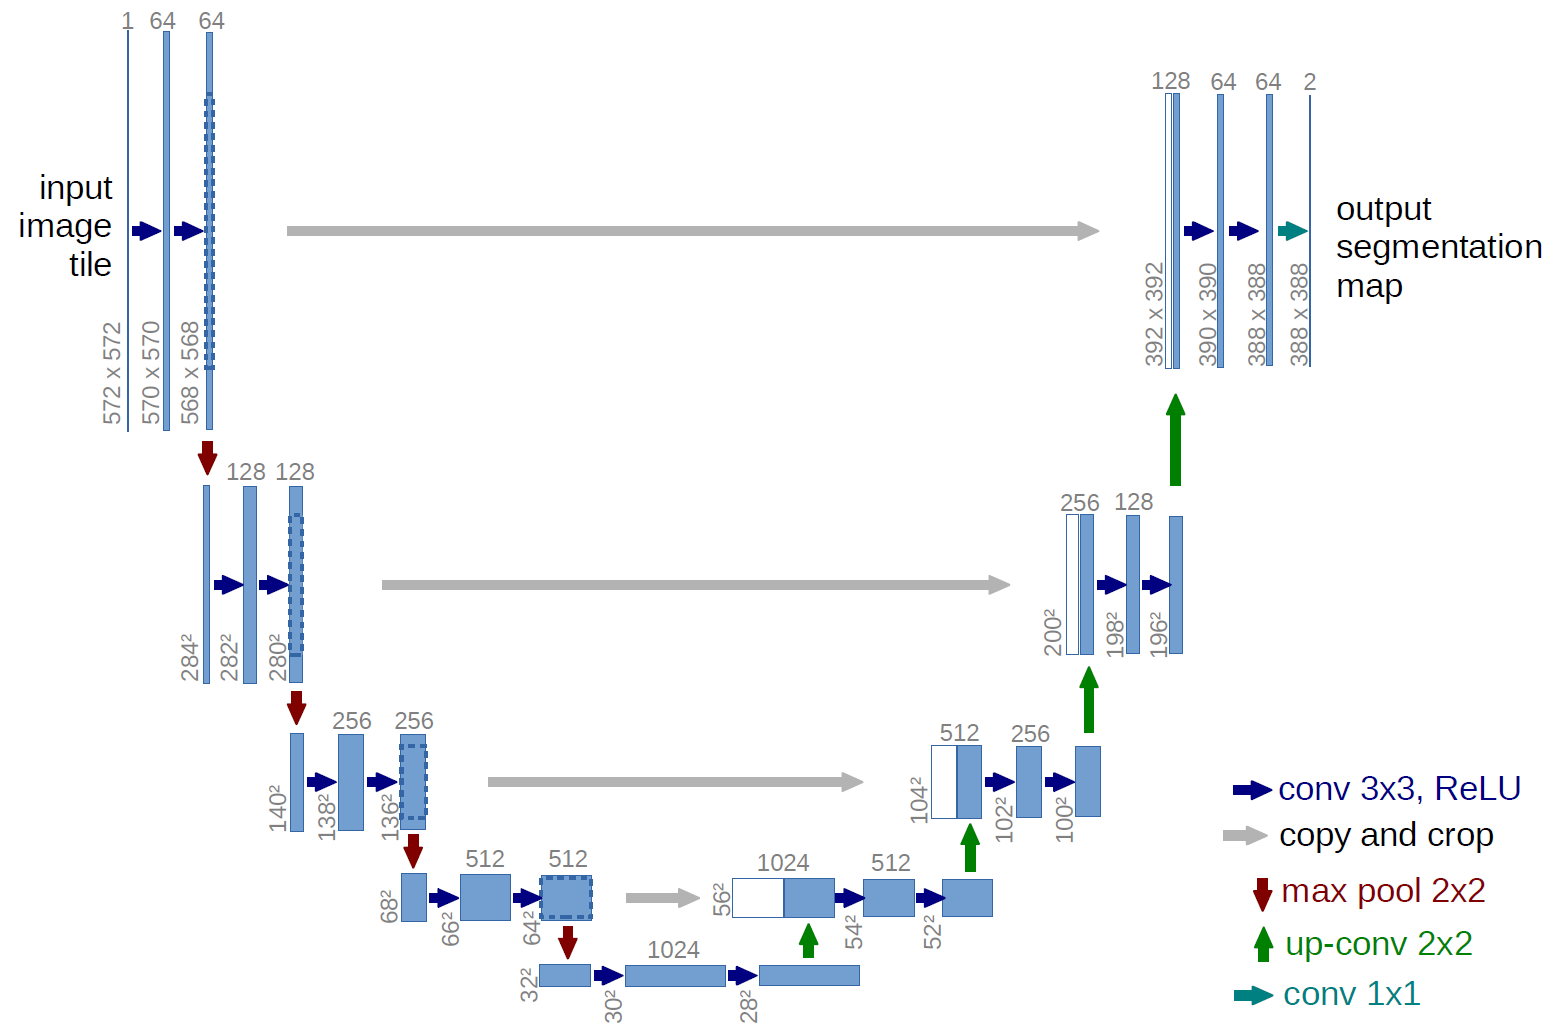
\includegraphics[width=0.85\textwidth]{images/u-net-architecture.png}
    \caption{A graphical visualization of the UNET architecture that was proposed in \cite{ronneberger_unet}.}
    \label{fig:unet}
\end{figure}
The UNET architecture consists of two parts: an encoder and a decoder, as shown in figure \ref{fig:unet}. 
The encoder follows the typical structure of a CNN, with repeated blocks of two 3x3 convolutions followed by 
a Rectified Linear Unit (ReLU) and a 2x2 max pooling operation with stride 2 for downsampling. At each 
downsampling step, the number of feature channels is doubled. \newline
The decoder is symmetric to the encoder, with repeated blocks of two 3x3 convolutions followed by a ReLU and 
a 2x2 up-convolution that halves the number of feature channels and upsamples the feature maps. The up-convolution is implemented by a 
transposed convolution or a bilinear interpolation followed by a 1x1 convolution.
One of the key features of UNET is the skip connections that connect the corresponding layers in the encoder 
and the decoder. These skip connections allow the decoder to use both high-level semantic features and 
low-level spatial features from the encoder, which helps to preserve the fine-grained details of the image 
and improve the segmentation accuracy.\newline
The final layer of UNET is a 1x1 convolution that maps each feature vector to the desired number of classes.
\section{Denoising Diffusion Probabilistic Model}
\label{sec:ddpm}
First, the intuition will be described, followed by the formal definition of a diffusion model. A diffusion probabilistic model or short "diffusion model" is described as a parameterized Markov chain \cite{ho_denoising_2020}. It is trained using variational interference. The goal is to produce matching data samples after a finite time. Starting with noise $x_\mathrm{T}$ the model produces less and less noisy samples $x_\mathrm{T-1} , x_\mathrm{T-2} , ...$. The end of this process results in an authentic sample $x_\mathrm{0}$. Each $t \in [0,T]$ resembles a timestamp that describes a certain noise-image-ratio for an image $x_\mathrm{0}$ and a noise $\epsilon$.  A diffusion model learns to synthesis less noised samples $x_\mathrm{t-1}$ from $x_\mathrm{t}$ by predicting the noise component of $x_\mathrm{t}$. This model is parameterized in \cite{ho_denoising_2020} as function $\epsilon_\mathrm{\theta}(x_\mathrm{t}, t)$.
\begin{figure}
    \centering
    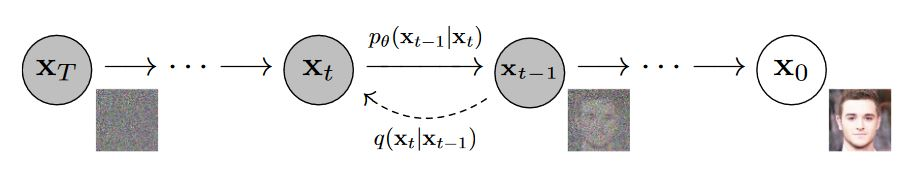
\includegraphics[width=\textwidth]{images/ddpm.JPG}
    \caption{A graphical representation of the noising- and denoising-process.}
    \label{fig:ddpm}
\end{figure}
Training this model is achieved by randomly fetching a data sample $x_\mathrm{0}$, a random timestamp $t$ and a noise $\epsilon$. \newline These result in $x_\mathrm{t}$ using formula \ref{eq:1}, presented in \cite{ho_denoising_2020}. $\beta_\mathrm{t}$ represents a variance schedule that describes the Gaussian noise added to $x_\mathrm{0}$ for $t \in [0,T]$.
\begin{equation}
\label{eq:1}
    q(x_\mathrm{t}|x_{t-1}) = \mathcal{N}(x_\mathrm{t};\sqrt{1-\beta_\mathrm{t}}x_\mathrm{t-1},\beta_\mathrm{t}\mathrm{I}).
\end{equation}
Instead of gradually adding noise over time 1 to T $q(x_\mathrm{t}|x_0)$ can be expressed as a Gaussian distribution with $\alpha:= 1-\beta_\mathrm{t}$ and $\overline{\alpha}_\mathrm{t} := \prod_\mathrm{s=0}^\mathrm{t} \alpha_\mathrm{s}$. The new formula that forms is

\begin{equation}
\label{eq:2}
    q(x_\mathrm{t}|x_0) = \mathcal{N}(x_\mathrm{t};\sqrt{\overline{\alpha}_\mathrm{t}}x_0,(1-\overline{\alpha}_\mathrm{t})\mathrm{I}) \newline 
\end{equation}
\begin{equation}
\label{eq:3}
        = \sqrt{\overline{\alpha}_\mathrm{t}}x_0 + \epsilon\sqrt{1-\overline{\alpha}_\mathrm{t}}, \epsilon\sim \mathcal{N}(0,\mathrm{I}).
\end{equation}
The objective of the training is a simple mean-squared error ${\|\epsilon_\theta(x_\mathrm{t},t)-\epsilon\|}^2$ minimization between the true noise and the predicted noise of the model.\newline \noindent Using the noise predictor $\epsilon_{\theta}(x_\mathrm{t}, t)$ sampling can be achieved. Sampling with a diffusion model is a repeated prediction of $x_\mathrm{t-1}$ from $x_\mathrm{t}$, starting at a randomly initialized $x_\mathrm{T}$. Under reasonable assumptions, using the Bayes theorem, the posterior $q(x_\mathrm{t-1}|x_\mathrm{t},x_0)$ is also a Gaussian with mean-function $\tilde{\mu}(x_\mathrm{t},x_0)$ and fixed variance $\tilde{\beta}_\mathrm{t}$ \cite{nichol_improved_2021}. 
\begin{equation}
\label{eq:4}
    \tilde{\mu}(x_\mathrm{t},x_0):= \frac{\sqrt{\overline{\alpha}_\mathrm{t-1}}\beta_\mathrm{t}}{1-\overline{\alpha}_\mathrm{t}}x_0 + \frac{\sqrt{\alpha_\mathrm{t}}(1-\overline{\alpha}_\mathrm{t-1})}{1-\overline{\alpha}_\mathrm{t}}x_\mathrm{t}
\end{equation}
\begin{equation}
\label{eq:5}
    \tilde{\beta}_\mathrm{t} := \frac{1-\overline{\alpha}_\mathrm{t-1}}{1-\overline{\alpha}_\mathrm{t}}\beta_\mathrm{t}
\end{equation}
\begin{equation}
\label{eq:6}
    q(x_\mathrm{t-1}|x_\mathrm{t},x_0) = \mathcal{N}(x_\mathrm{t-1}; \tilde{\mu}(x_\mathrm{t},x_0),\tilde{\beta}_\mathrm{t}\mathrm{I})
\end{equation}
Theoretically, sampling from $q(x_0)$ works by first sampling from $q(x_\mathrm{T})$ and then sample the reverse steps $q(x_\mathrm{t-1}|x_\mathrm{t})$ until $x_0$ is reached. Reasonable settings for $\beta_\mathrm{t}$ and \(T\) provide trivial sampling for $x_\mathrm{T}$, because the distribution $q(x_\mathrm{T})$ is nearly an isotropic Gaussian distribution \cite{dhariwal_diffusion_2021}.\newline \noindent
After establishing all necessary steps, an approximation of $q(x_\mathrm{t-1}|x_\mathrm{t})$ is missing. Using a neural network to predict mean $\mu_\theta$ and a diagonal covariance matrix $\Sigma_\theta$ is considered. This is possible because \cite{sohl-dickstein_deep_2015} notes that the distribution $q(x_\mathrm{t-1}|x_\mathrm{t})$ approaches a diagonal Gaussian distribution for $T \rightarrow \infty$, which corresponds to $\beta_\mathrm{t} \rightarrow 0$.
\begin{equation}
\label{eq:7}
    p_\theta(x_\mathrm{t-1}|x_\mathrm{t}) := \mathcal{N}(x_\mathrm{t-1};\mu_\theta(x_\mathrm{t},t),\Sigma_\theta(x_\mathrm{t},t))
\end{equation}
The model goal is to learn the true data distribution $q(x_0)$. In \cite{ho_denoising_2020} it is shown that a different objective produces better samples in general. Therefore they don't directly predict $\mu_\theta(x_\mathrm{t},t)$ with a neural network, but rather $\epsilon_{\theta}(x_\mathrm{t}, t)$ so it matches the noise $\epsilon$  used in \ref{eq:3}. During the sampling process, $\mu_\theta(x_\mathrm{t},t)$ can be derived from $\epsilon_{\theta}(x_\mathrm{t}, t)$ by substitution:
\begin{equation}
\label{eq:8}
    \mu_\theta(x_\mathrm{t},t) = \frac{1}{\sqrt{\alpha_\mathrm{t}}}\left(x_\mathrm{t} - \frac{1-\alpha_\mathrm{t}}{\sqrt{1-\overline{\alpha}_\mathrm{t}}}\epsilon_{\theta}(x,t)\right)
\end{equation}
This mathematical foundations are put to use at different data structures to create generative models. The following chapters contain two contexts of generative models using DDPMs.
\newpage
\section{Maximum Mean Discrepancy}
\label{sec:mmd}
The maximum mean discrepancy (MMD) \cite{gretton2008kernel} is a statistical indicator that can be used to determine how close to each other underlying sample distributions are.
A small MMD indicates high similarity. This can be used in generative models to compare synthetic sample sets with real sample sets.
Decent MMD scores can so be used to argue that models perform good in the the task of synthesizing the real data distribution.\newline
In practice, the squared difference between the two sets is considered as presented in \cite{esteban2017realvalued}.
The assumptions that they introduce and the operations that are performed result in a score that can be used to estimate the quality of 
a generative model.\newline \newline
\resizebox{\textwidth}{!}{$\widehat{\textbf{MMD}}^{2} = \frac{1}{n(n-1)}\sum_{i=1}^{n}\sum_{j\neq i}^{n}K(x_{i},x_{j})-
\frac{2}{mn}\sum_{i=1}^{n}\sum_{j= 1}^{m}K(x_{i},y_{j})+
\frac{1}{m(m-1)}\sum_{i=1}^{m}\sum_{j\neq i}^{m}K(y_{i},y_{j})$} \newline\newline
Where $K:X \times Y \rightarrow \mathbb{R} $ is a given kernel and $\{x_{i}\}^{D_{real}}_{i=1}$,
$\{y_{j}\}^{D_{fake}}_{j=1}$ are real and synthetic samples.
\section{t-SNE}
\label{sec:tsne}
One method used for evaluation is the t-distributed stochastic neighbor embedding (t-SNE), which is employed for visualization proposed in \cite{maaten2008tsne}.
t-SNE is a method that maps high dimensional data samples into a two- or three-dimensional embedding. First it computes probabilities proportional to the similarity of each data points on the high dimensional representation. Afterwards it tries to find lower dimensional representations by minimization of the Kullback-Leibler divergence.\newline
In the end the lower dimensional data points can be visualized in a scatterplot, e.g. seen in \ref{fig:tsne example}.
t-SNE is interesting for this thesis because time series data, in comparison to image data, is not simply evaluated by looking at a time series graph. Having a visualization method holds great benefits for understanding since it tranforms high dimensional time series data into an interpretable representation for humans.
\begin{figure}[h!]
    \centering
    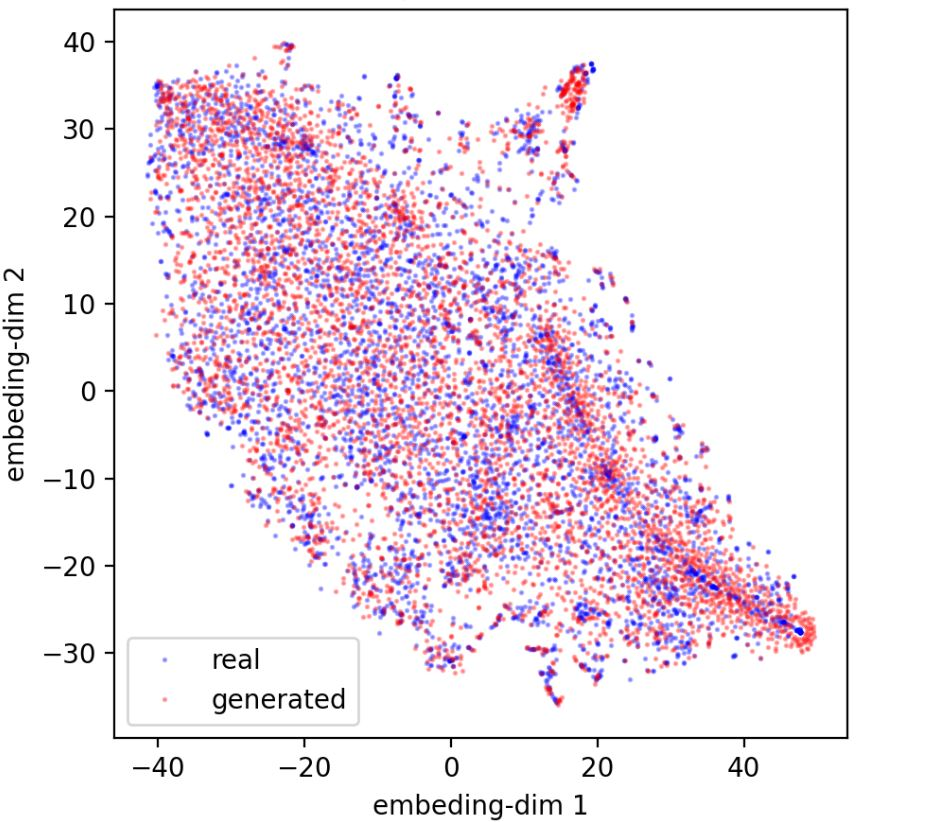
\includegraphics[width=0.75\textwidth]{images/tsne example.JPG}
    \caption{An example of an t-SNE plot where two distributions of time series data were embedded.}
    \label{fig:tsne example}
\end{figure}
\newpage
\section{Continual Learning}
\label{sec:cont learning}
Continual Learning (CL) is the question whether intelligent agents are capable of containing/remembering 
knowledge through different sample distribution that are given to the model iteratively in multiple distinguished training cycles.
It can be described as lifelong training with changing sample distributions which the agent must learn without losing performance on past data distributions.
One effect that occurs during continual learning scenarios is known as catastrophic forgetting \cite{wang2023comprehensive}. 
This term describes a model that is gradually getting worse at older tasks that it learned during its lifetime. To prevent this effect different methods and approaches were investigated. In \cite{wang2023comprehensive} a variety of different CL approaches. Those can be seen in figure \ref{fig:cl_tax}.
\begin{figure}[h!]
    \centering
    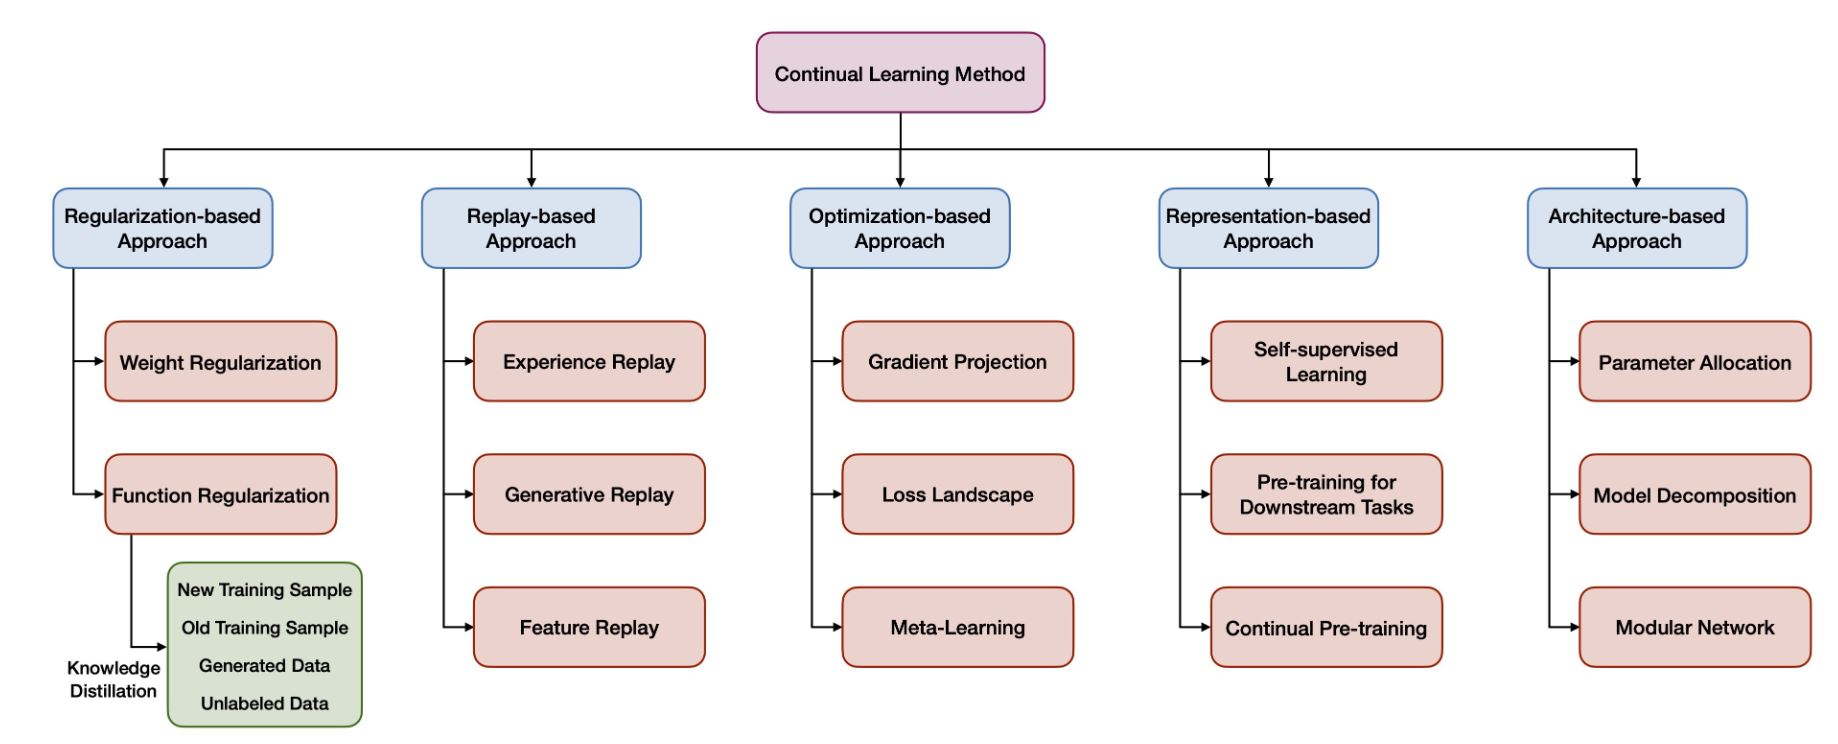
\includegraphics[width=\textwidth]{images/cl_taxonomie.JPG}
    \caption{A state-of-the-art and elaborated taxonomy of representative continual learning methods found in \cite{wang2023comprehensive}.}
    \label{fig:cl_tax}
\end{figure}
\chapter{State of the Art}
\label{sec:stateoftheart}
DDPMs emerged first in a thermodynamic context \cite{sohl-dickstein_deep_2015} and were improved and developed since then. 
Publications like \cite{ho_denoising_2020}, \cite{dhariwal_diffusion_2021} and \cite{nichol_improved_2021} were published in 
less than a year from one another and laid the foundation for many popular applications today. It is a rather young field of research and 
major breakthroughs occur regularly. The main focus of the majority of research paper regarding DDPM focus on the domain of image data and computer vision.
Searching for specific DDPM models that work with time series data is most of the time not met with success. Still there are many different approaches for utilization of DDPM in the context of time series data. For example found in \cite{rasul2021autoregressive} as an autoregressive approach for time series forecasting.


\chapter{Approach}
\label{sec:approach}
\section{From Images to Time Series}
\label{sec:from images to time series}
After establishing a solid foundation regarding the inner workings of DDPM in section \ref{sec:ddpm}, this knowledge was applied to define the necessary operations and methods. This enabled the construction of a working DDPM for testing and evaluation.\newline
Very beneficial is the fact, that the overall mathematical semantic of the equations described in \ref{sec:ddpm} does not need to be changed
just some technical changes to the shapes of the matrices, that are multiplied, to guarantee the right output forms was made.
After incorporating these changes the forward process could be performed and visualized as seen in fig. \ref{fig:time series ddpm process}.
Using images the forward process or the noising of an image can be understood intuitively. The same effect can now be achieved by looking at the
noised time series. The last step if the noising process resembles just random noise, while the intermediate steps still hold some characteristics.\newline
After establishing the forward process noised sampling can be performed which empowers us to define an 
efficient training cycle. Before a model is trained, the first step involves defining the underlying architecture that will predict the noise used in the backward process.
\begin{figure}
    \centering
    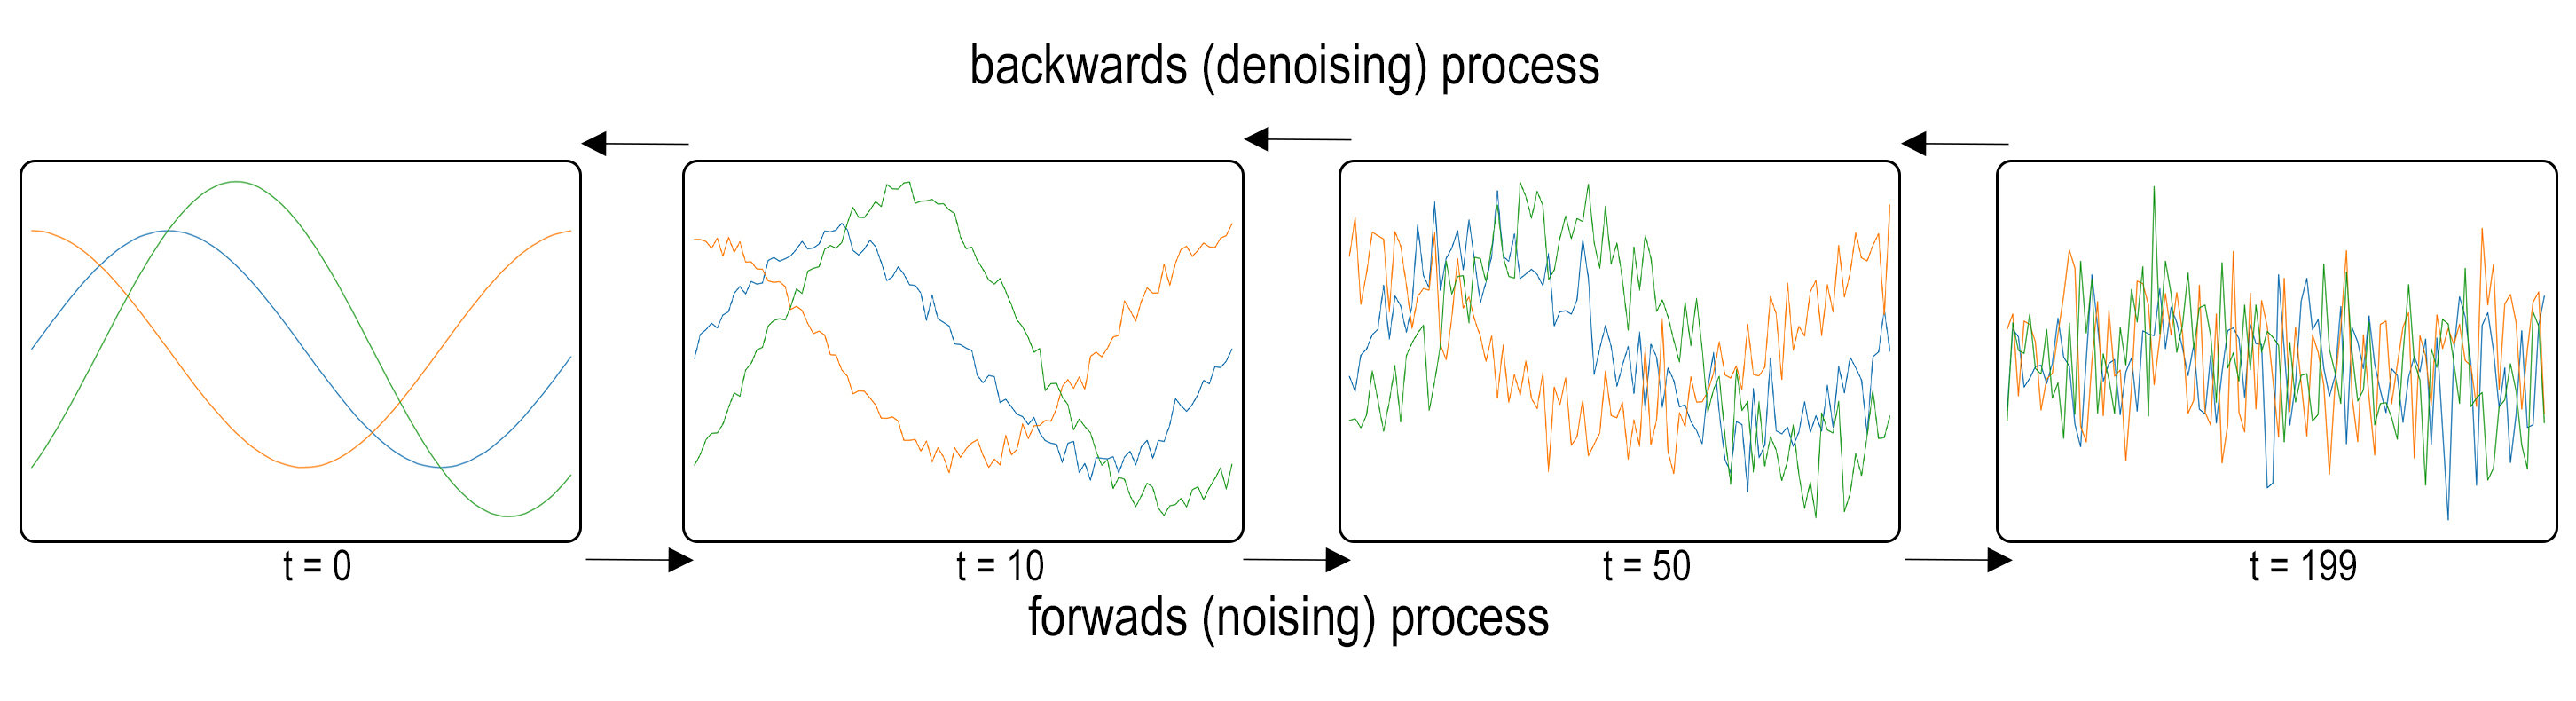
\includegraphics[width=\textwidth]{images/noised time series.jpg}
    \caption{Visualization of the forward/backwards process of a DDPM for time series samples with T = 200 using different sin/cos waves.}
    \label{fig:time series ddpm process}
\end{figure}
\section{UNET for Time Series}
\label{sec:unet time series}
The UNET architecture, as described in \ref{sec:unet}, was taken, and it was restructured to function with 1-D time series data. Mostly, this was achieved by replacing 2-D convolutional and 2-D transposed convolutional 
layers with the corresponding 1-D variants. The underlying structure of our UNET can be visualized by figure \ref{fig:unet} just that it takes 1D input samples instead of 2D images as already mentioned.\newline
After establishing the base structure, additions to the UNET that differ from the original setup are also defined. One of those
additions are self attention layers after every up-/downsampling block. Also these blocks take an extra parameters
as input - a timestamp. This is the timestamp that is defined in the DDPM operations in section \ref{sec:ddpm}. Before going into the UNET this timestamp
is positionally encoded. After that the timestamp is embedded linearly in the convolutions. So in every up-/downsampling block the model retains information about the current step in the noising/denoising process.\newline
Conditional dependencies in the form of an entity embedding \cite{guo2016entity} were also added to the UNET. This embedding allows us to embed categorical and continual information that can also be provided to the UNET to guarantee
a more controlled generative process. The model can produce samples that correspond to a specific time of the year or resemble certain sample features like average temperature. The embedding dimensions are chosen in a way so that the 
dimension of the positional encoding of the timestamp match. Those two embeddings are added afterwards to form a new timestamp that now also holds contextual information about the sample in every block. 
\begin{figure}
    \centering
    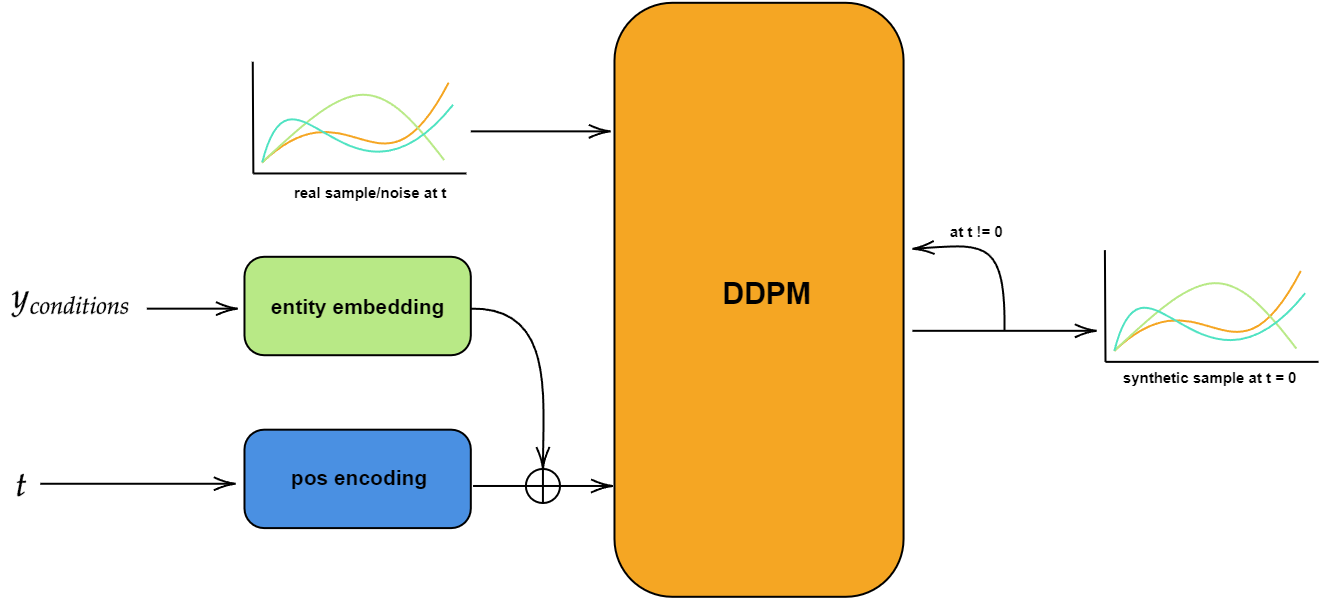
\includegraphics[width=\textwidth]{images/unet1d.png}
    \caption{Visualization of the DDPM process used in this project.}
    \label{fig:unet1d}
\end{figure}
The entire process can be visualized as seen in fig. \ref{fig:unet1d}. The embeddings are simultaneously trained with the model and can be saved and frozen for later usage in other models.
\section{Uni- and Multivariate}
\label{sec: uni and multi}
The until now described architecture are capable of learning/sampling different dimensions of data.
In the field of generative image models this can be easy understood by different color channels. On a more general scale it can be
understood as a multiple target task. The models are trained to synthesize multiple features at the same time. As an example time series data samples are presented. Models that are used in a energy domain mostly focus on some form of "power-delivered" feature they are mostly 
interested in. A univariate model will e.g. now only generate those power time series samples. A Multivariate approach could also 
include learning and synthesizing the temperature and fuel/electricity price time series. In the real world the underlying problem and demand for
a spectrum is bigger so Multivariate approaches seem more attractive. Also they could bring a performance boost by providing more sequential 
context through other features during the training process, which means that the model learns to generate features in relation to and with each other.
These additional features could be already included in the dataset. Examples could be temperature, price of electricity or sun intensity.
But 'virtual' features could be also defined. Such virtual features could be a daily sine or cosine graph that maps a single timestamp in a day to a tuple of sine/cosine values.
For better understanding a sample was taken from an experiment defined at section \ref{sec:experiments}. In figure \ref{fig:multivar example} you can see a real featuer kW and two virtual ones.
\begin{figure}[h!]
    \centering
    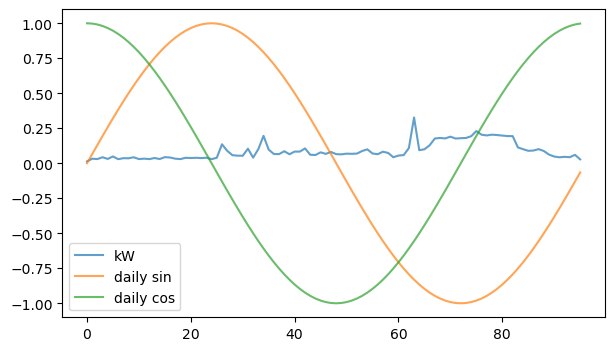
\includegraphics[width=0.6\textwidth]{images/multivar_example.png}
    \caption{A multivariate sample containing kW,daily sin and daily cos as dimensions.}
    \label{fig:multivar example}
\end{figure}

\chapter{Datasets}
\label{sec:datasets}
In this chapter, the definition of experimental datasets is presented. These datasets exhibit various characteristics that our models aim to capture. The following sections provide a general overview of the source, size, and other elements that require consideration.
Three distinct datasets related to the energy domain, particularly in the context of time series data, were considered for our experiments. The primary focus, especially for the univariate approaches outlined in section \ref{sec: uni and multi}, was a form of 'power delivered.' For the multivariate approaches, additional features were also considered, if available, and virtual features were established, such as a daily sine or cosine.
All three datasets are open-source, and this section will describe the original state of the datasets. Additionally, details about how feature columns were added, excluded, or transformed will be discussed.
\subsection*{London Smart Meter dataset}
\label{subsec:LSM}
The London Smart Meter Dataset \cite{LSMsource} contains energy consumption readings for a set of 5,567 London Households that took part in the UK Power Networks led Low Carbon London project between November 2011 and February 2014.
Readings were taken at half hourly intervals. The customers in the trial were recruited as a balanced sample representative of the Greater London population.
The dataset contains energy consumption, in kWh (per half hour), unique household identifier, date and time. No further feature extraction steps were performed. Only the virtual samples described in section \ref{sec: uni and multi} were added. Moreover, the unique IDs, as previously mentioned, were utilized as categorical conditions, while weekly/yearly sine and cosine values served as continual conditions for our entity embedding, as described in section \ref{sec:unet time series}.
An overview of all parameters can be seen in table \ref{table:lsm params}. In figure \ref{fig:one_year_lsm} a year of a randomly picked household is shown. One year is depicted for a randomly sampled household and also a rolling mean of one week (336 timestamps).\newline
\begin{figure}
    \centering
    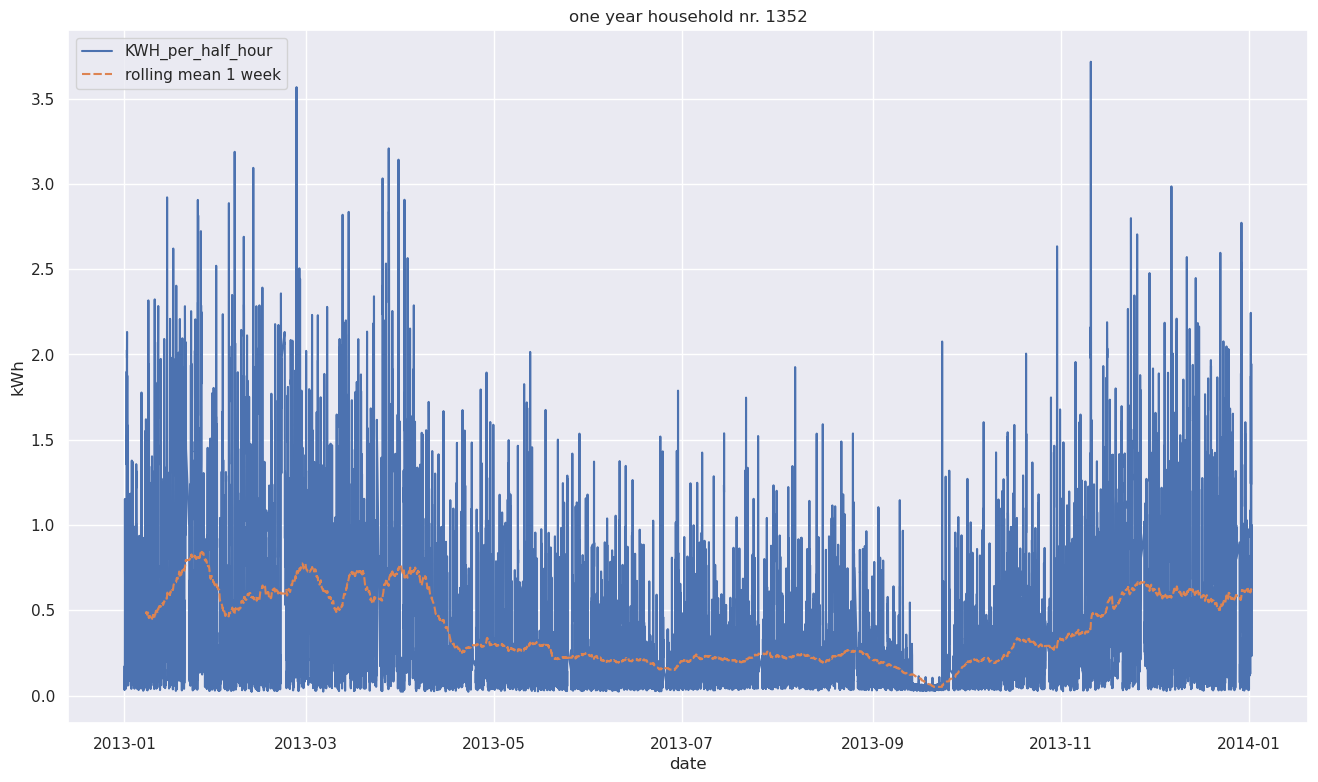
\includegraphics[width = \textwidth]{images/one_year_rm_lsm1357.png}
    \caption{Power consumption of a randomly picked LSM household for one year and a rolling mean for one week.}
    \label{fig:one_year_lsm}
\end{figure}
\begin{table}[h!]
    \centering
    \begin{tabular}{|c c c c c c|} 
         \hline
         name & dtype & type & univariate & multivariate & augmentation\\ [0.5ex] 
         \hline\hline
         kWperhalfhour & float & time series & \checkmark & \checkmark & normalized\\ 
         \hline
         daily sine & float & time series & - & \checkmark & -\\ 
         \hline
         daily cosine & float & time series & - & \checkmark & -\\ 
         \hline
         weekly sine & float & continual & \checkmark & \checkmark & - \\ 
         \hline
         weekly cosine & float & continual & \checkmark & \checkmark & -\\ 
         \hline
         yearly sine & float & continual & \checkmark & \checkmark & -\\ 
         \hline
         yearly cosine & float & continual & \checkmark & \checkmark & -\\ 
         \hline
         household ID & string & categorical & \checkmark & \checkmark & label encoded\\ 
         \hline
        \end{tabular}
    \caption{Overview of different targets and conditional data used for London Smart Meter Experiments.}
    \label{table:lsm params}
\end{table}

\subsection*{OpenMeter dataset} 
\label{subsec:openemter}
Open Meter \cite{OMsource} is a open platform where people, communes or institutions provide data about their power usage. This power is measured in watt in a 15-min resolution.
Providers also leave information about the usage, how much area their household or business occupies and location information to narrow down geographical context in Germany.
Open Meter also provides weather data for almost all sensors which can also be added to the training. During experiments categorical conditions city and post code are taken into consideration as well as area, weekly/yearly sine and weekly/yearly cosine for continual conditions. We also added the daily sine, daily cosine and temperature as targets for the multivariate approach.
An overview of all parameters can be seen in table \ref{table:openmeter params}.\newline
\begin{figure}[!h]
    \centering
    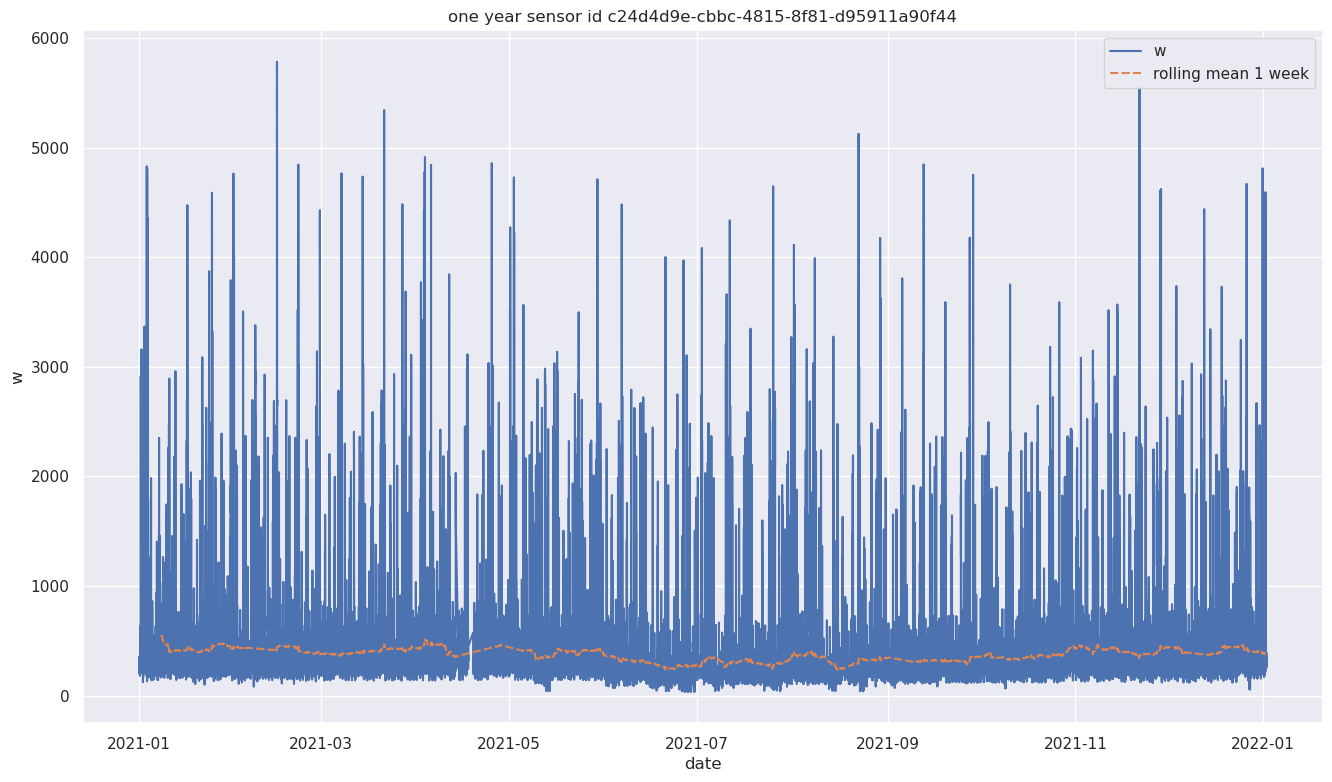
\includegraphics[width = \textwidth]{images/one_year_rolling_mean_om.png}
    \caption{Power consumption of a randomly picked OpenMeter sensor for one year and a rolling mean for one week.}
    \label{fig:one_year_lsm}
\end{figure}
\begin{table}[!h]
    \centering
    \begin{tabular}{|c c c c c c|}
         \hline
         name & dtype & type & univariate & multivariate & augmentation\\ [0.5ex] 
         \hline\hline
         power used & float & time series & \checkmark & \checkmark & normalized\\ 
         \hline
         temperature & float & time series & - & \checkmark & normalized\\ 
         \hline
         daily sine & float & time series & - & \checkmark & -\\ 
         \hline
         daily cosine & float & time series & - & \checkmark & -\\ 
         \hline
         weekly sine & float & continual & \checkmark & \checkmark & -\\ 
         \hline
         weekly cosine & float & continual & \checkmark & \checkmark & -\\ 
         \hline
         yearly sine & float & continual & \checkmark & \checkmark & -\\ 
         \hline
         yearly cosine & float & continual & \checkmark & \checkmark & -\\ 
         \hline
         area & float & continual & \checkmark & \checkmark & label encoded\\ 
         \hline
         city & string & categorical & \checkmark & \checkmark & label encoded\\ 
         \hline
         post code & string & categorical & \checkmark & \checkmark & label encoded\\ 
         \hline
        \end{tabular}
    \caption{Overview of different targets and conditional data used for Open Meter Experiments.}
    \label{table:openmeter params}
\end{table}
\newpage
\subsection*{ACN dataset}
\label{subsec:ACN}
The Adaptive Charging Network (ACN) Dataset \cite{ACNsource} provides information about electrical vehicle (EV) charging sessions. Gathered at different sites (caltech, jpl and office) that contain multiple charging stations.
The original dataset contained mostly technical information about the power delivery and time of occupation. The data was expanded by incorporating weather information, such as temperature and humidity. Also some feature crafting was performed to 
create fields like chargingTime, parkingTime and idleTime. All fields considered can be seen in table \ref{table:acn params}.
\begin{table}[h!]
    \centering
    \begin{tabular}{|c c c c|} 
         \hline
         name & dtype & type  & augmentation\\ [0.5ex] 
         \hline\hline
         kWhDelivered & float & time series  & normalized\\ 
         \hline
         chargingTime & float & time series  & normalized\\ 
         \hline
         idleTime & float & time series   & normalized\\ 
         \hline
         Temperature & float & time series   & normalized\\ 
         \hline
         2 metre relative humidity & float & time series   & normalized\\ 
         \hline
         2 metre specific humidity & float & time series   & normalized\\ 
         \hline
         weekly sine & float & continual   & -\\ 
         \hline
         weekly cosine & float & continual   & -\\ 
         \hline
         yearly sine & float & continual   & -\\ 
         \hline
         yearly cosine & float & continual   & -\\ 
         \hline
         siteType & float & categorical   & label encoded\\ 
         \hline
        \end{tabular}
    \caption{Overview of different targets and conditional data used for ACN Experiments.}
    \label{table:acn params}
\end{table}
For the ACN dataset we decided to directly synthesize multivariate data so there won't be a distinction during evaluation.
The final dataset we used was derived from combining the ACN caltech site dataset with the ACN jpl site dataset. 
\begin{figure}[h!]
    \centering
    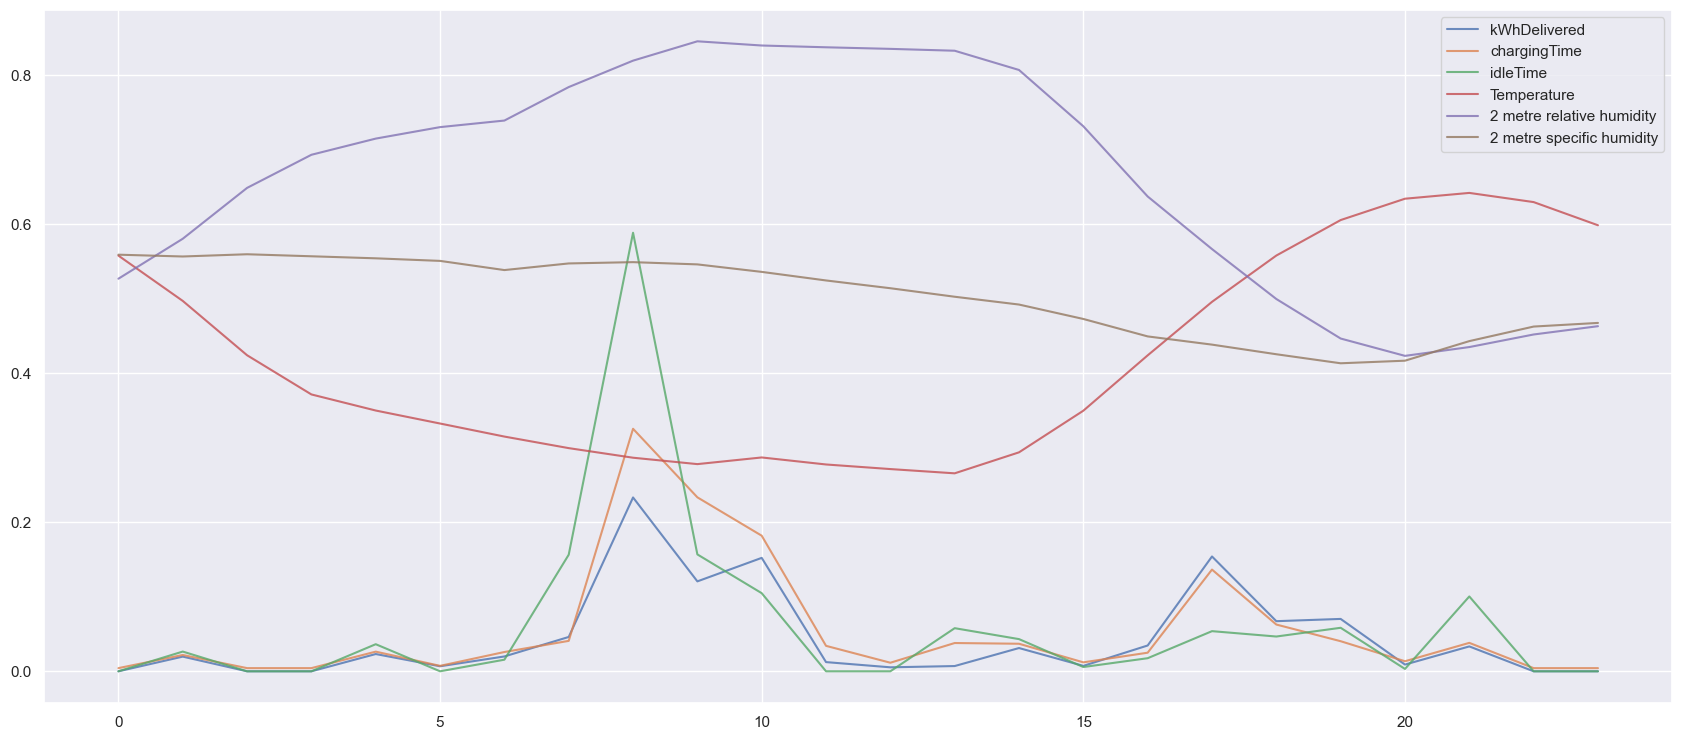
\includegraphics[width=\textwidth]{images/acn_sample.png}
    \caption{A multivariate sample from the ACN dataset.}
    \label{fig:ACN sample}
\end{figure}
\chapter{Experiments}
\label{sec:experiments}
In this chapter, the definition of various evaluation methods and scenarios performed at the end of training a model is presented. The choice of evaluation methods depends on the initial dataset used for training, as outlined in Chapter \ref{sec:datasets}.

\section{LSM experiments}
The LSM dataset is characterized by a wealth of unique households and a large volume of data samples, providing an opportunity for a comprehensive experimental setup for generative models.
5400 unique households were taken and split into batches of 100 households. We then train the model on the current batch, synthesize samples and then evaluate the quality with different statistical methods.
For instance, lsm 01 batch comprises households from 1 to 100 in the dataset, lsm 02 includes households from 101 to 200, and so forth. The resolution of the time was half hour measurements resulting in samples with 48 timestamps which corresponds to one day. Additionally, two different models were trained to examine the difference between uni- and multivariate models. Consequently, a total of 55 trained models were compared for univariate and 55 for multivariate approaches. The evaluation metrics included the MMD score, as described in section \ref{sec:mmd}, the t-SNE plot outlined in section \ref{sec:tsne}, and various visualizations of daily means, which were then compared to the real data.

\section{OpenMeter experiments}
In contrast to the LSM dataset, the OpenMeter dataset is not curated, and the overall quality of the samples is inconsistent. It exhibits issues such as missing values for different sensors, incoherent feature representation, among others. To facilitate better experimentation and comparability, we opted to define a smaller subset.
The subset includes only sensors categorized as 'private' (the other category being commercial/public), and is also limited to values recorded in the years 2021 and 2022. The sensors in the OpenMeter dataset have a resolution of 15-minute measurements, resulting in 96 values for one day. Univariate and multivariate models are compared, the MMD scores computed, t-SNE plots discussed and daily means for both real and synthetic samples analyzed.

\section{ACN experiments}
For the ACN dataset, a deliberate choice was made to adopt the multivariate approach, ensuring that metrics yield multiple results for each respective dimension. Consequently, daily means are examined for every dimension, the MMD score is computed for each dimension compared to the real data, and one t-SNE plot is discussed. In this case, the dimensional reduction of the t-SNE method can handle multivariate time series samples, allowing for analysis in a single plot.\newline
An applied test was also conducted, examining both real data and synthetic data in a continual learning scenario. Initially, the real data was subjected to testing, involving the training of an arbitrary forecasting model on three different sections corresponding to evenly spread 4-month parts of the initial 2019 jpl dataset. The model was trained using MSE as the loss and EWC, SI, and LWF as three regularization terms which are specific to continuous learning, more specifically regularization-based approaches. After each section, the forecasting performance was evaluated. One assumption was that the model might forget the pre-task of forecasting earlier sections or retain it throughout the experiments. The real data exhibited a certain performance for this continual learning task.Subsequently, the same experiment was replicated with a synthetic JPL dataset. This synthetic data also demonstrated a certain performance or behavior for the continual learning task. Ultimately, a comparison was made, suggesting that the synthetic data behaves similarly to the real data, serving as another indication of good synthetic sample quality. Important to notice is that the following results do not answer the question whether the continual learning performance can be enhanced by involving synthetic data. This is a task for future work which is discussed in section \ref{sec:apply cl}. The applied experiments and their results presented were conducted by Yuan Wang, another student at the IES group. This thesis just discusses the results.
\chapter{Results}
\label{sec:results}
In this chapter, the results for the experimental setups defined in the previous chapter are discussed.
\section{Training Configurations and Architecture}
\label{sec:training config}
As with other neural network architectures, DDPM rely on a certain configuration of parameters that can influence the training results tremendously.
Through extensive testing and experimenting, the seemingly best parameters were narrowed down. 
They were used for all datasets and evaluation tests. 
\begin{table}[h!]
    \centering
    \begin{tabular}{|c c c c c |} 
         \hline
         $\beta_{min}$ & $\beta_{max}$ & $T$ & batch size & learning rate\\ [0.5ex] 
         \hline\hline
         $10^{-6}$ & 0.02 & \{200,250\} & 32 & $10^{-3}$ \\ 
         \hline
        \end{tabular}
    \caption{Parameters for training and setting up DDPMs.}
    \label{table:params}
\end{table}
The parameters depicted in table \ref{table:params} produced the most promising results. 
For the ACN dataset, a value of 250 was chosen for T, as 200 time steps were not sufficient to produce fully denoised samples.
\section{LSM results}
\label{subsec:LSM res}
After training the models we generate a set of 5000 synthetic samples that are compared against 5000 real samples from the corresponding LSM batch. 
Doing so we can compare different results for all statistical indicators and calculate averages.
\begin{figure}[!h]
    \centering
    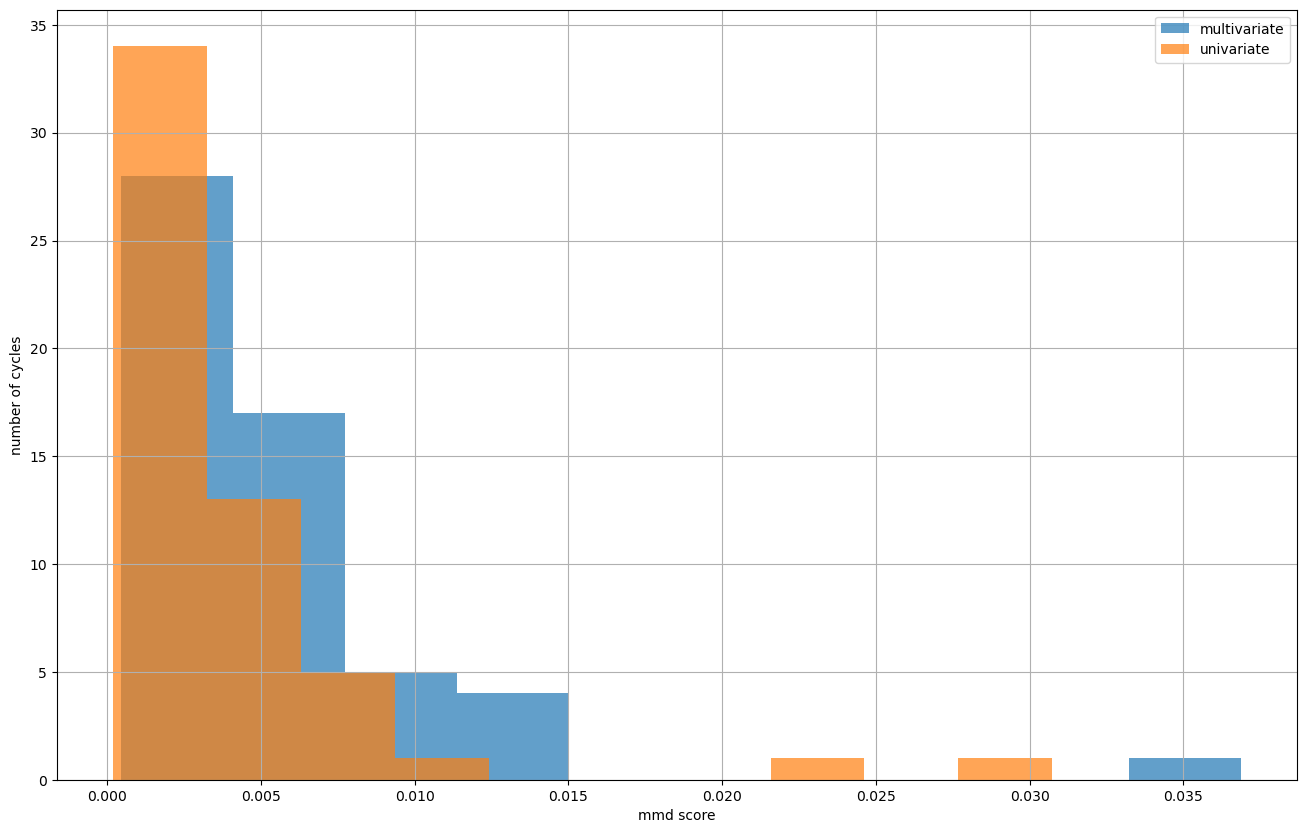
\includegraphics[width=\textwidth]{images/lsm_res_histo.png}
    \caption{Histogram of all values seen in table \ref{table:lsm results}.}
    \label{fig:lsm res histo}
\end{figure}
In Table \ref{table:lsm results}, the results for the MMD score, as described in section \ref{sec:mmd}, are presented. Both uni- and multivariate approaches yield decent results. Notably, the univariate approach, which focuses solely on synthesizing the kWhDelivered feature, demonstrates slightly better outcomes. This is evident when comparing the means, with $mean_{uni} = 0.003569$ and $mean_{multi} = 0.005349$. Additionally, a histogram of both result sets can be examined in Figure \ref{fig:lsm res histo}.\newline
In figure \ref{fig:tsne overall uni} and figure \ref{fig:tsne overall mult} t-SNE plots are depicted for all batches, as described in section \ref{sec:tsne}. Again a comparison of 5000 real and 5000 generated samples is made.
In summary, it can be concluded that the overlapping of all t-SNE plots suggests that both uni- and multivariate models performed decently.\newline
The MMD score and the t-SNE plots are used to get a statistical certainty about the quality of the data. Another venue that can be explored are visualizations that can be understood by the human eye. Therefore we look at daily means and compare them to the generated samples. Having a similar structures might be another hint for good model quality. In the following plots a comparison of characteristic days is conducted. Showing all 55 household batches is possible, but a decission was made to show only four randomly picked batches for the sake of simplicity. As seen in fig. \ref{fig:sample mean 22} the daily mean of the overall real households was picked up by the model. For more information other figures \ref{fig:sample mean 09}, \ref{fig:sample mean 37} and  \ref{fig:sample mean 53} can be seen under the Appendix section.
\begin{figure}
    \centering
    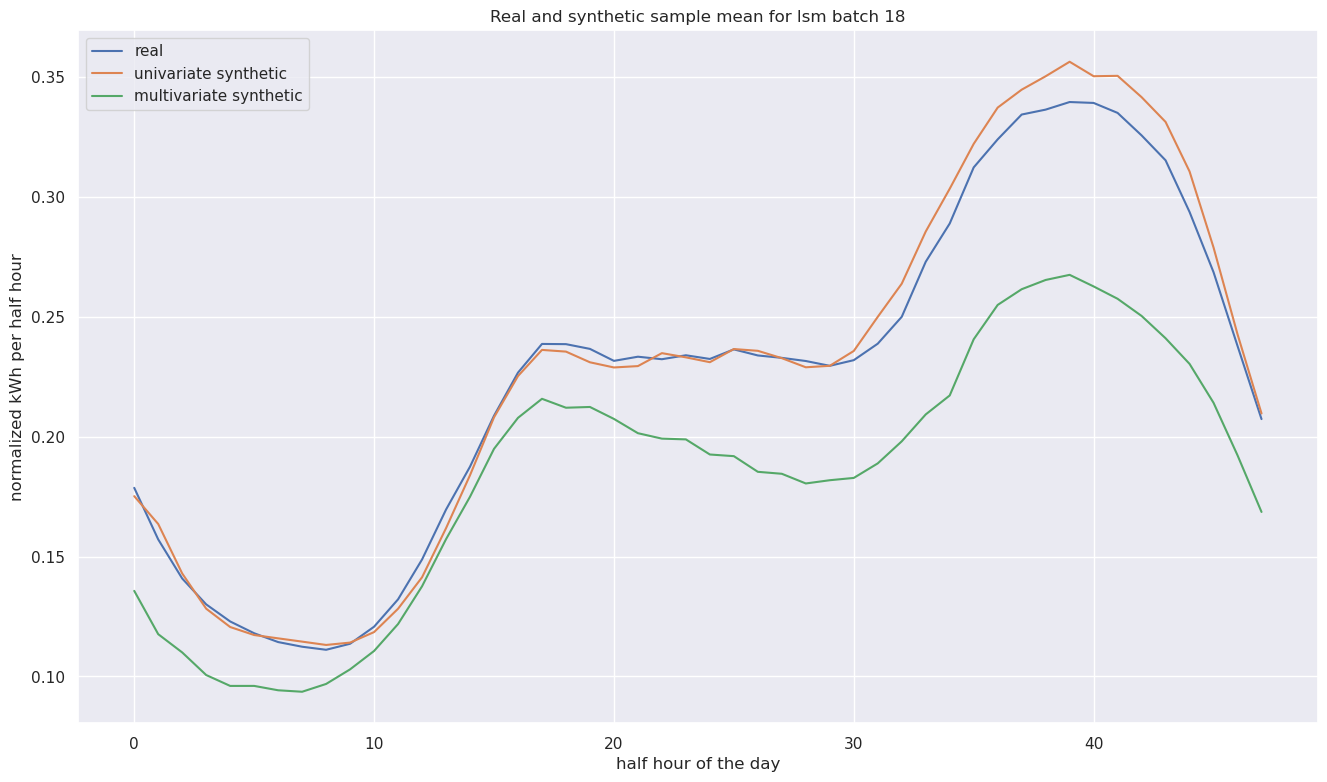
\includegraphics[width=\textwidth]{images/lsm_dm_18.png}
    \caption{Real and generated sample daily mean for lsm batch 18}
    \label{fig:sample mean 22}
\end{figure}

\section{Openmeter results}
\label{subsec:OM res}
After training, 5000 synthetic samples and 5000 randomly selected real samples were sampled to perform MMD scoring and t-SNE plots. Additionally, daily mean plots comparing real and synthetic data are presented in Figure \ref{fig:om dm}. Although differences are noticeable between all three graphs, the overall trend of the data was captured accurately. The MMD scores can be seen in Table \ref{table:om results}.
\begin{figure}
    \centering
    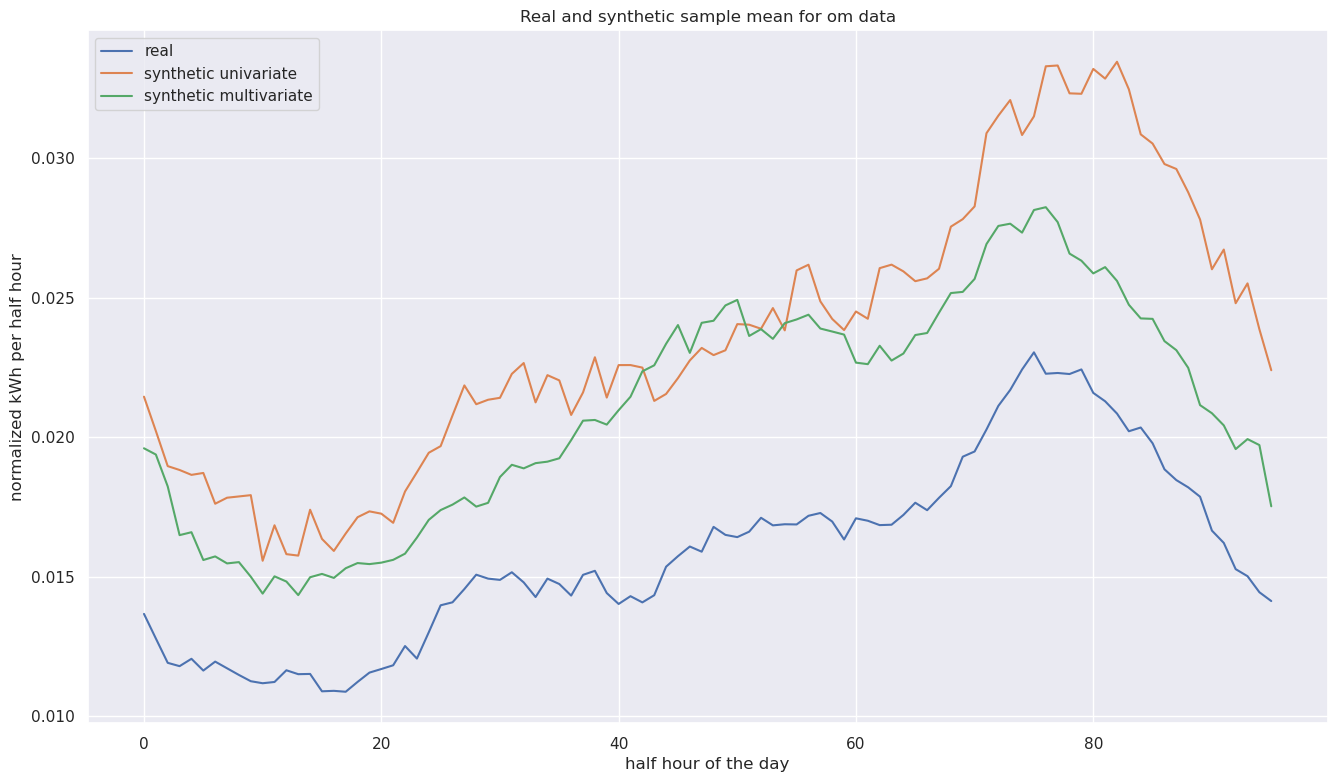
\includegraphics[width=\textwidth]{images/om_dm_private.png}
    \caption{Real and generated sample daily mean for om private data}
    \label{fig:om dm}
\end{figure}
\begin{table}[h!]
    \centering
    \begin{tabular}{|c | c c|}
        \hline
         & univariate & multivariate\\
        \hline\hline
        mmd score & 0.033825 & 0.074251\\
        \hline
    \end{tabular}
    \caption{Results for the uni-/multivariate openmeter experiments.}
    \label{table:om results}
\end{table}
The t-SNE plots can be examined in figures \ref{fig:om tsne multi} and \ref{fig:om tsne uni}. The mmd-scores suggest that the multivariate approach performed worse. The t-SNE on the other hand doesn't suggest a clear successor. Overall it can be argued that the complexity of synthesizing more features can have a negative impact on the overall quality but further experiments need to be performed to verify or falsify this assumption.
Multivariate models are non the less better due to the fact that they produce a spectrum of targets which is more likely for a real world scenario where many different time series are useful.
\section{ACN results}
\label{subsec:ACN res}
In the combined plots seen in figures \ref{fig:all acn} all daily means of the different channels can be seen. They are reconstructed almost identically.
\begin{figure}
\begin{subfigure}{.45\textwidth}
  \centering
  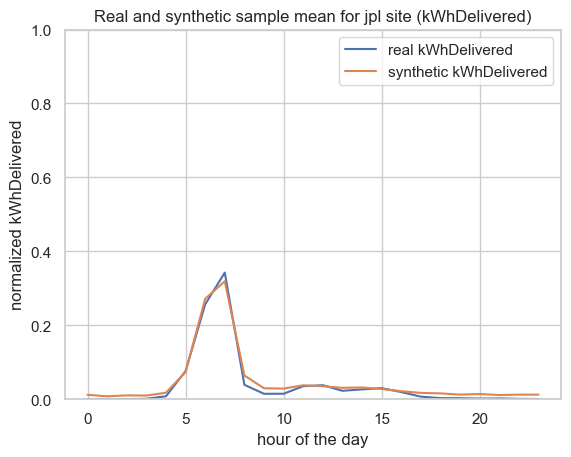
\includegraphics[width=.8\linewidth]{images/jpl_day_mean_kwh.png}
  \caption{Real and synthetic daily mean for kWhDelivered.}
  \label{fig:kwh}
\end{subfigure}
\hfill
\begin{subfigure}{.45\textwidth}
  \centering
  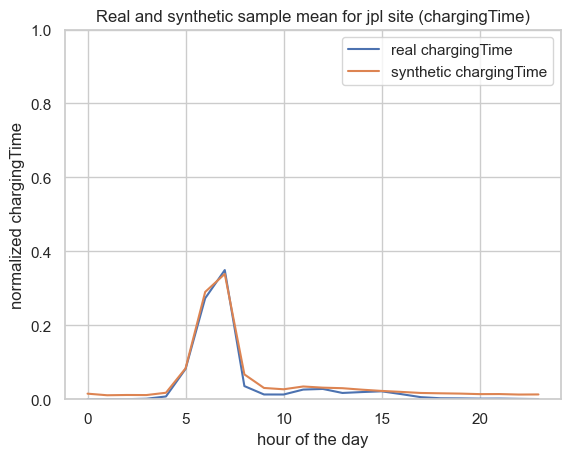
\includegraphics[width=.8\linewidth]{images/jpl_day_mean_ct.png}
  \caption{Real and synthetic daily mean for chargingTime.}
  \label{fig:ct}
\end{subfigure}
\begin{subfigure}{.45\textwidth}
  \centering
  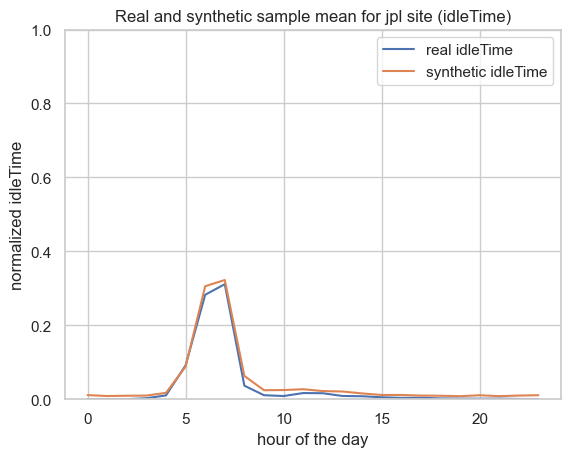
\includegraphics[width=.8\linewidth]{images/jpl_day_mean_it.png}
  \caption{Real and synthetic daily mean for idleTime.}
  \label{fig:kwh}
\end{subfigure}
\hfill
\begin{subfigure}{.45\textwidth}
  \centering
  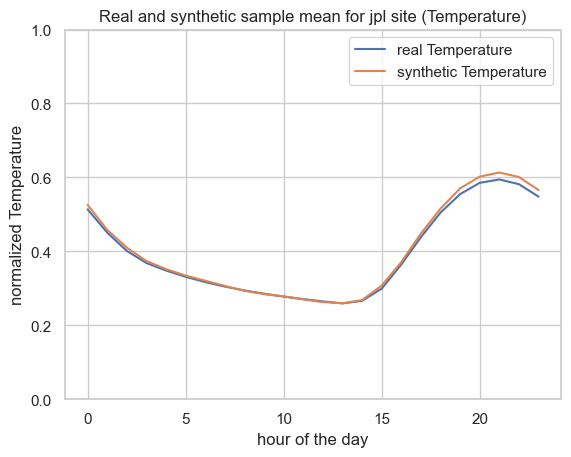
\includegraphics[width=.8\linewidth]{images/jpl_day_mean_temp.png}
  \caption{Real and synthetic daily mean for temperature.}
  \label{fig:ct}
\end{subfigure}
\begin{subfigure}{.45\textwidth}
  \centering
  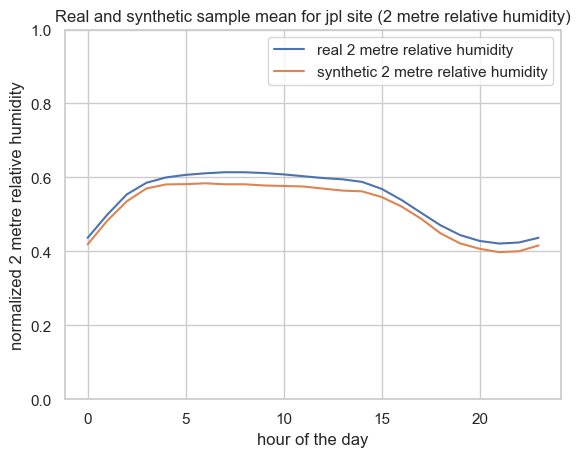
\includegraphics[width=.8\linewidth]{images/jpl_day_mean_rhum.png}
  \caption{Real and synthetic daily mean for relative humidity.}
  \label{fig:kwh}
\end{subfigure}
\hfill
\begin{subfigure}{.45\textwidth}
  \centering
  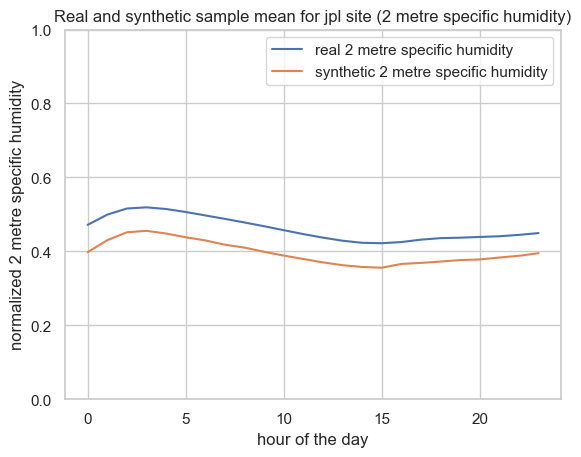
\includegraphics[width=.8\linewidth]{images/jpl_day_mean_shum.png}
  \caption{Real and synthetic daily mean for specific humidity.}
  \label{fig:ct}
\end{subfigure}
\caption{Real and synthetic daily mean for all multivariate time series features.}
\label{fig:all acn}
\end{figure}

\begin{table}[h!]
    \centering
    \begin{tabular}{|c | c  |}
        \hline
         &mmd score\\
        \hline\hline
         kWhDelivered&0.014720\\
         chargingTime&0.016854\\
         idleTime&0.008288\\ 
         Temperature&0.003077\\
         relative humidity&0.014960\\
         specific humidity&0.029262 \\
        \hline
    \end{tabular}
    \caption{Results for the multivariate ACN experiments.}
    \label{table:om results}
\end{table}%
Generally the overall data richness of the ACN dataset was significantly smaller in comparison to the LSM and OpenMeter dataset. In the end only around 500 real samples to 500 synthetic ones are compared. In the other experiments 5000 for each group were compared. This is especially important when looking at the visualization through t-SNE. Obviously the significance of those results shrinks with less samples but can still be taken into consideration. In figure \ref{fig:tsne jpl} very good results for the synthetic jpl samples can be seen.
\begin{figure}[h!]
    \centering
    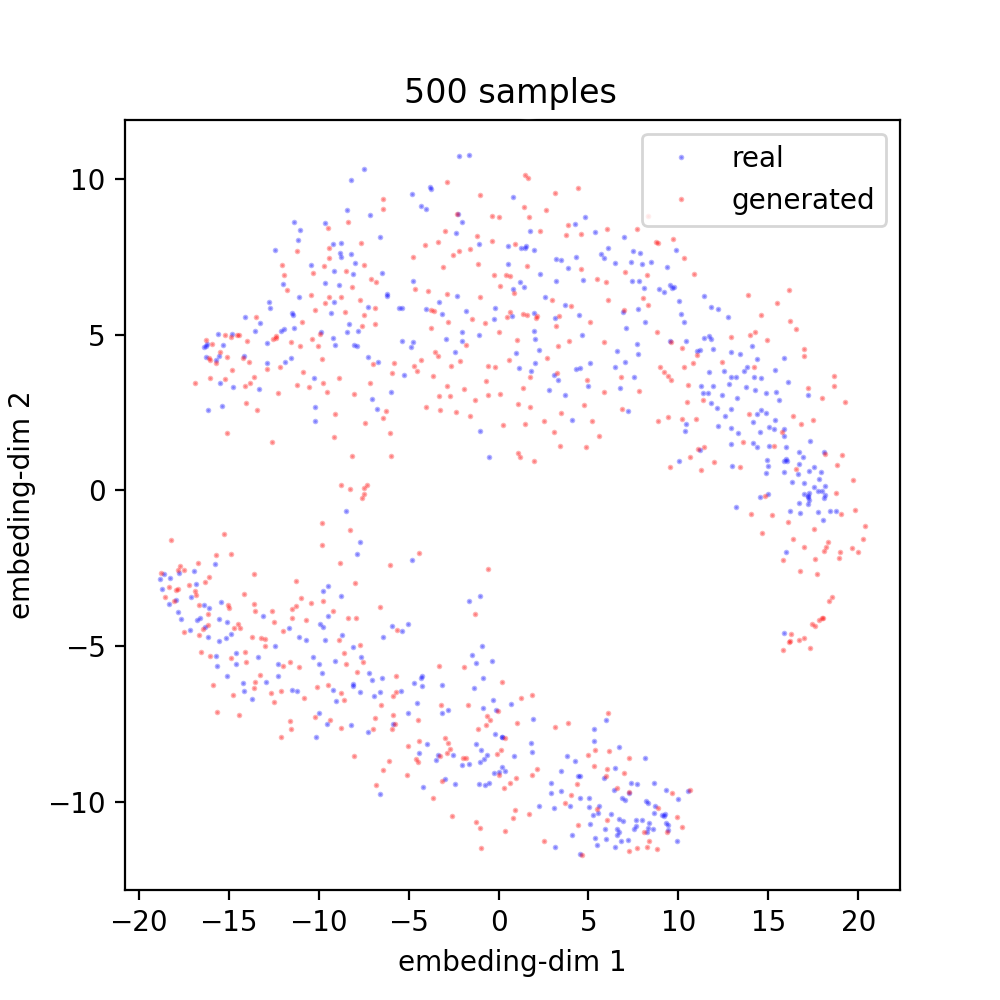
\includegraphics[width=0.6\textwidth]{images/jpl_tsne_res.png}
    \caption{t-SNE plot for 500 real and synthetic jpl site samples.}
    \label{fig:tsne jpl}
\end{figure}\newline \noindent
Finally, a look at a year of real and synthetic jpl site samples was made. A synthetic jpl site year with its rolling mean for one week is depicted in figure \ref{fig: jpl syntethic year}.
\begin{figure}[h!]
    \centering
    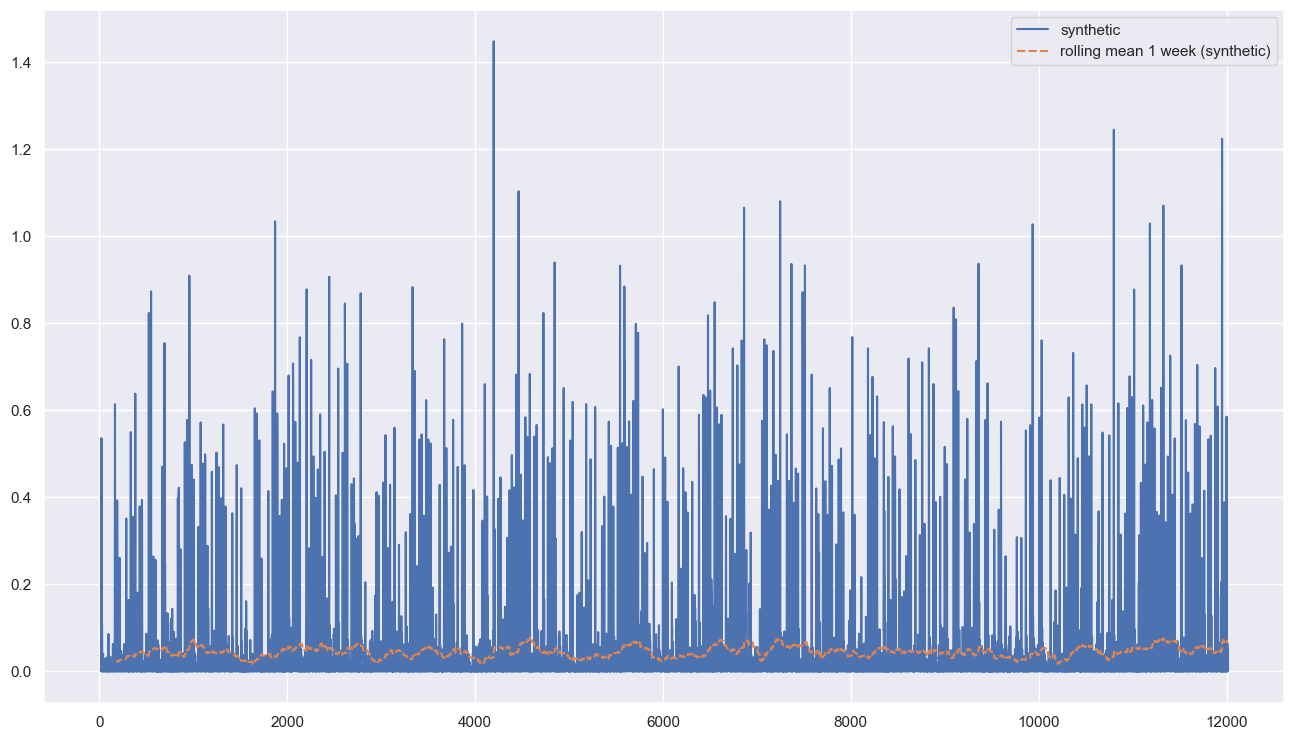
\includegraphics[width=\textwidth]{images/one_year_rm_jpl_synth.png}
    \caption{One year synthetic jpl site samples with rolling mean for one week (kWhDelivered).}
    \label{fig: jpl syntethic year}
\end{figure}\newline \noindent
Afterwards, the rolling mean for one week of one year real samples was taken and compared to the synthetic rolling mean for one week seen in figure \ref{fig: jpl year comp}.
\begin{figure}[h!]
    \centering
    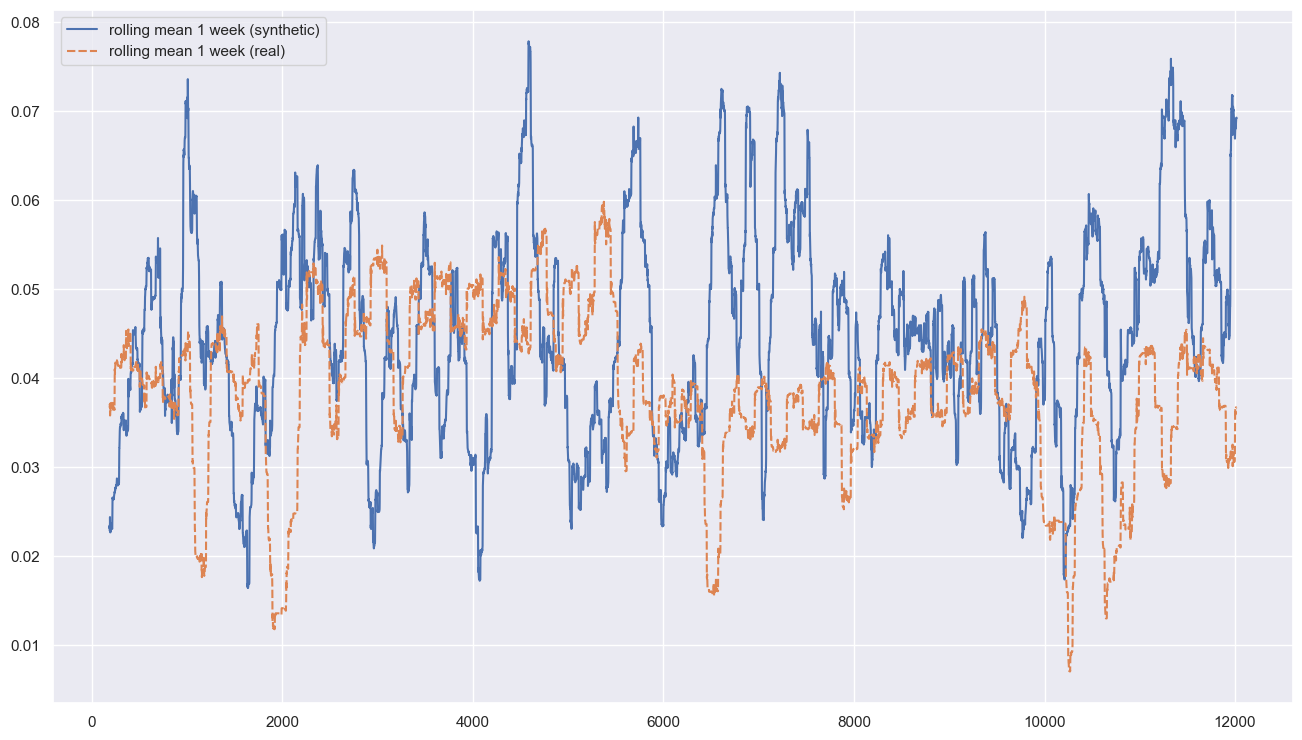
\includegraphics[width=\textwidth]{images/one_year_rm_jpl_1week_comp.png}
    \caption{One year synthetic jpl site rolling mean for one week compared to real jpl site year.}
    \label{fig: jpl year comp}
\end{figure}\newline \noindent
Overall the results look similar but on closer examination it is visible that differences especially for the comparison in figure \ref{fig: jpl year comp} occur.
The differences are small, ranging in the interval of +/- 0.04.\newline
Ultimatly, a discussion about the applicative test, that was defined in section \ref{sec:experiments} is presented. Only the results for EWC regularization terms are presented for the sake of simplicity, since all regularization terms performed similar. Looking at the following to figures \ref{fig:real forecast} and \ref{fig:synth forecast} both real and synthetic samples are shown and both were able to retain the continual learning task by still forecasting previous sections after going thru new training cycles for later sections. This similar behaviour of synthtetic and real data samples might suggest a good quality of the synthetic samples. Important to mention is that the plots do not cover four months as described when looking at the x-axis. The plots contain test samples after train/test splitting the four month datasets that make up the three sections.
\begin{figure}[h!]
    \centering
    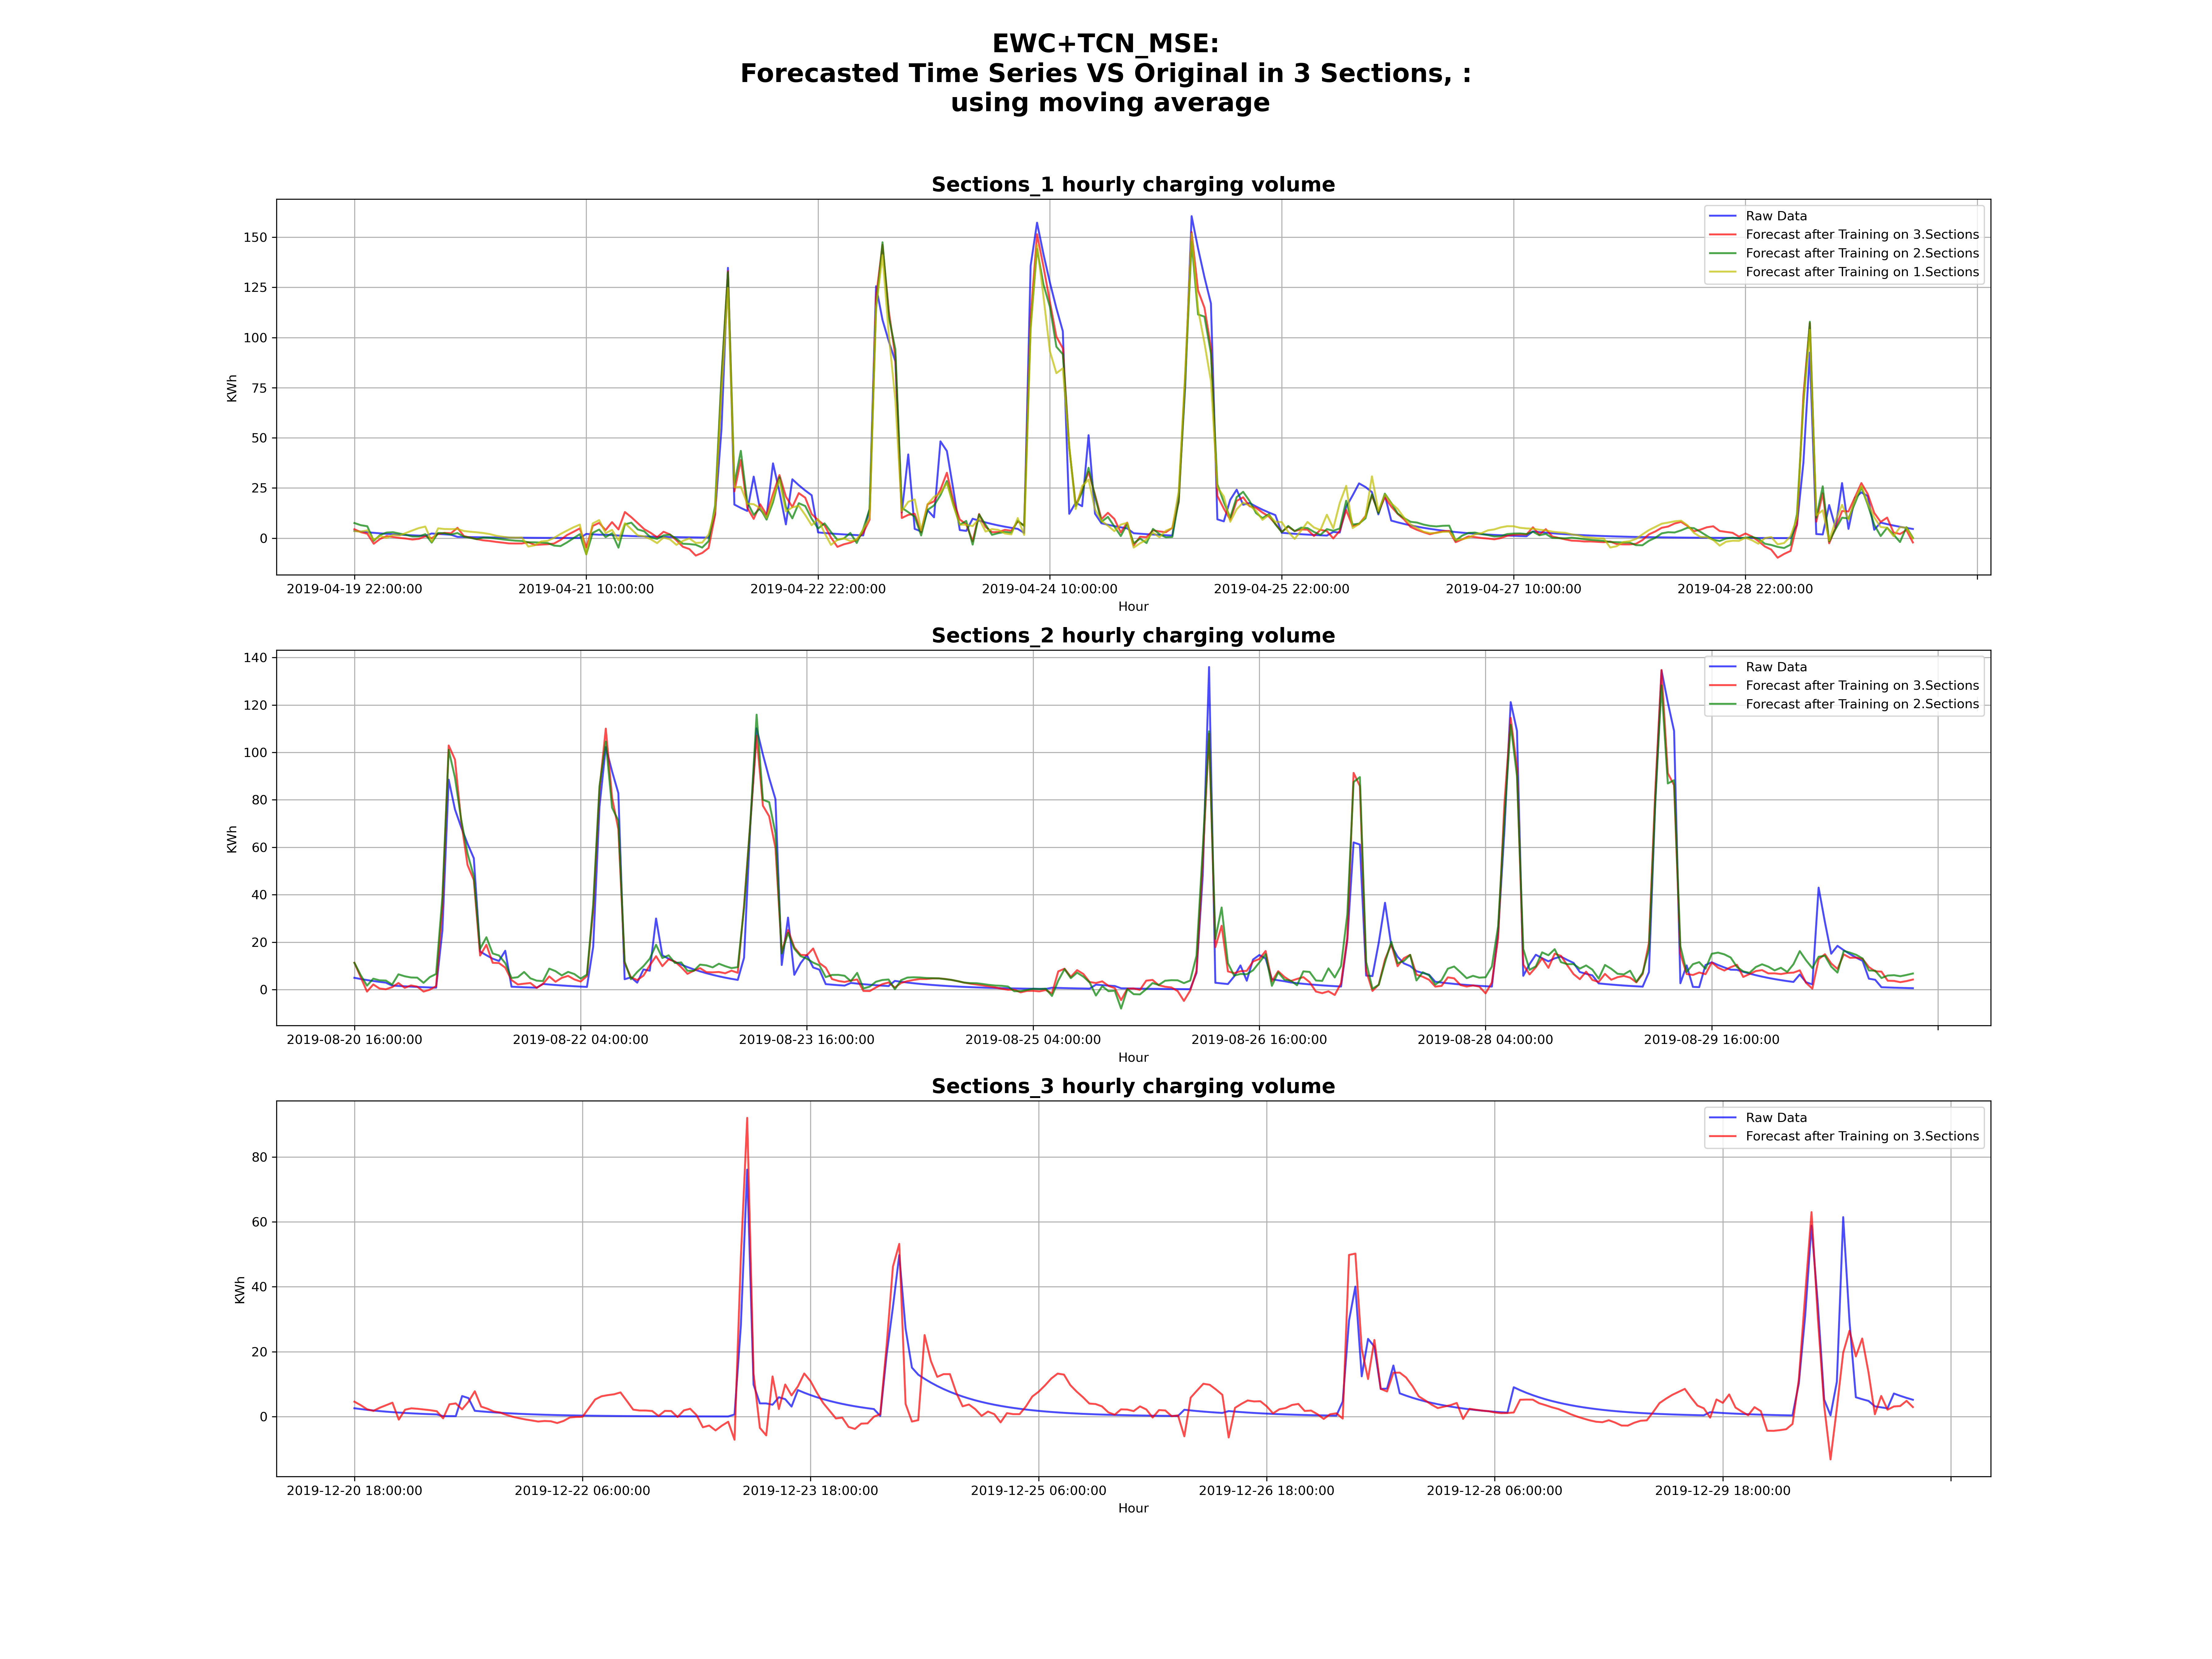
\includegraphics[width=.8\textwidth]{images/synthetic_real.png}
    \caption{CL experiment for real data jpl site samples (created by Yuan Wang).}
    \label{fig:real forecast}
\end{figure}
\begin{figure}[h!]
    \centering
    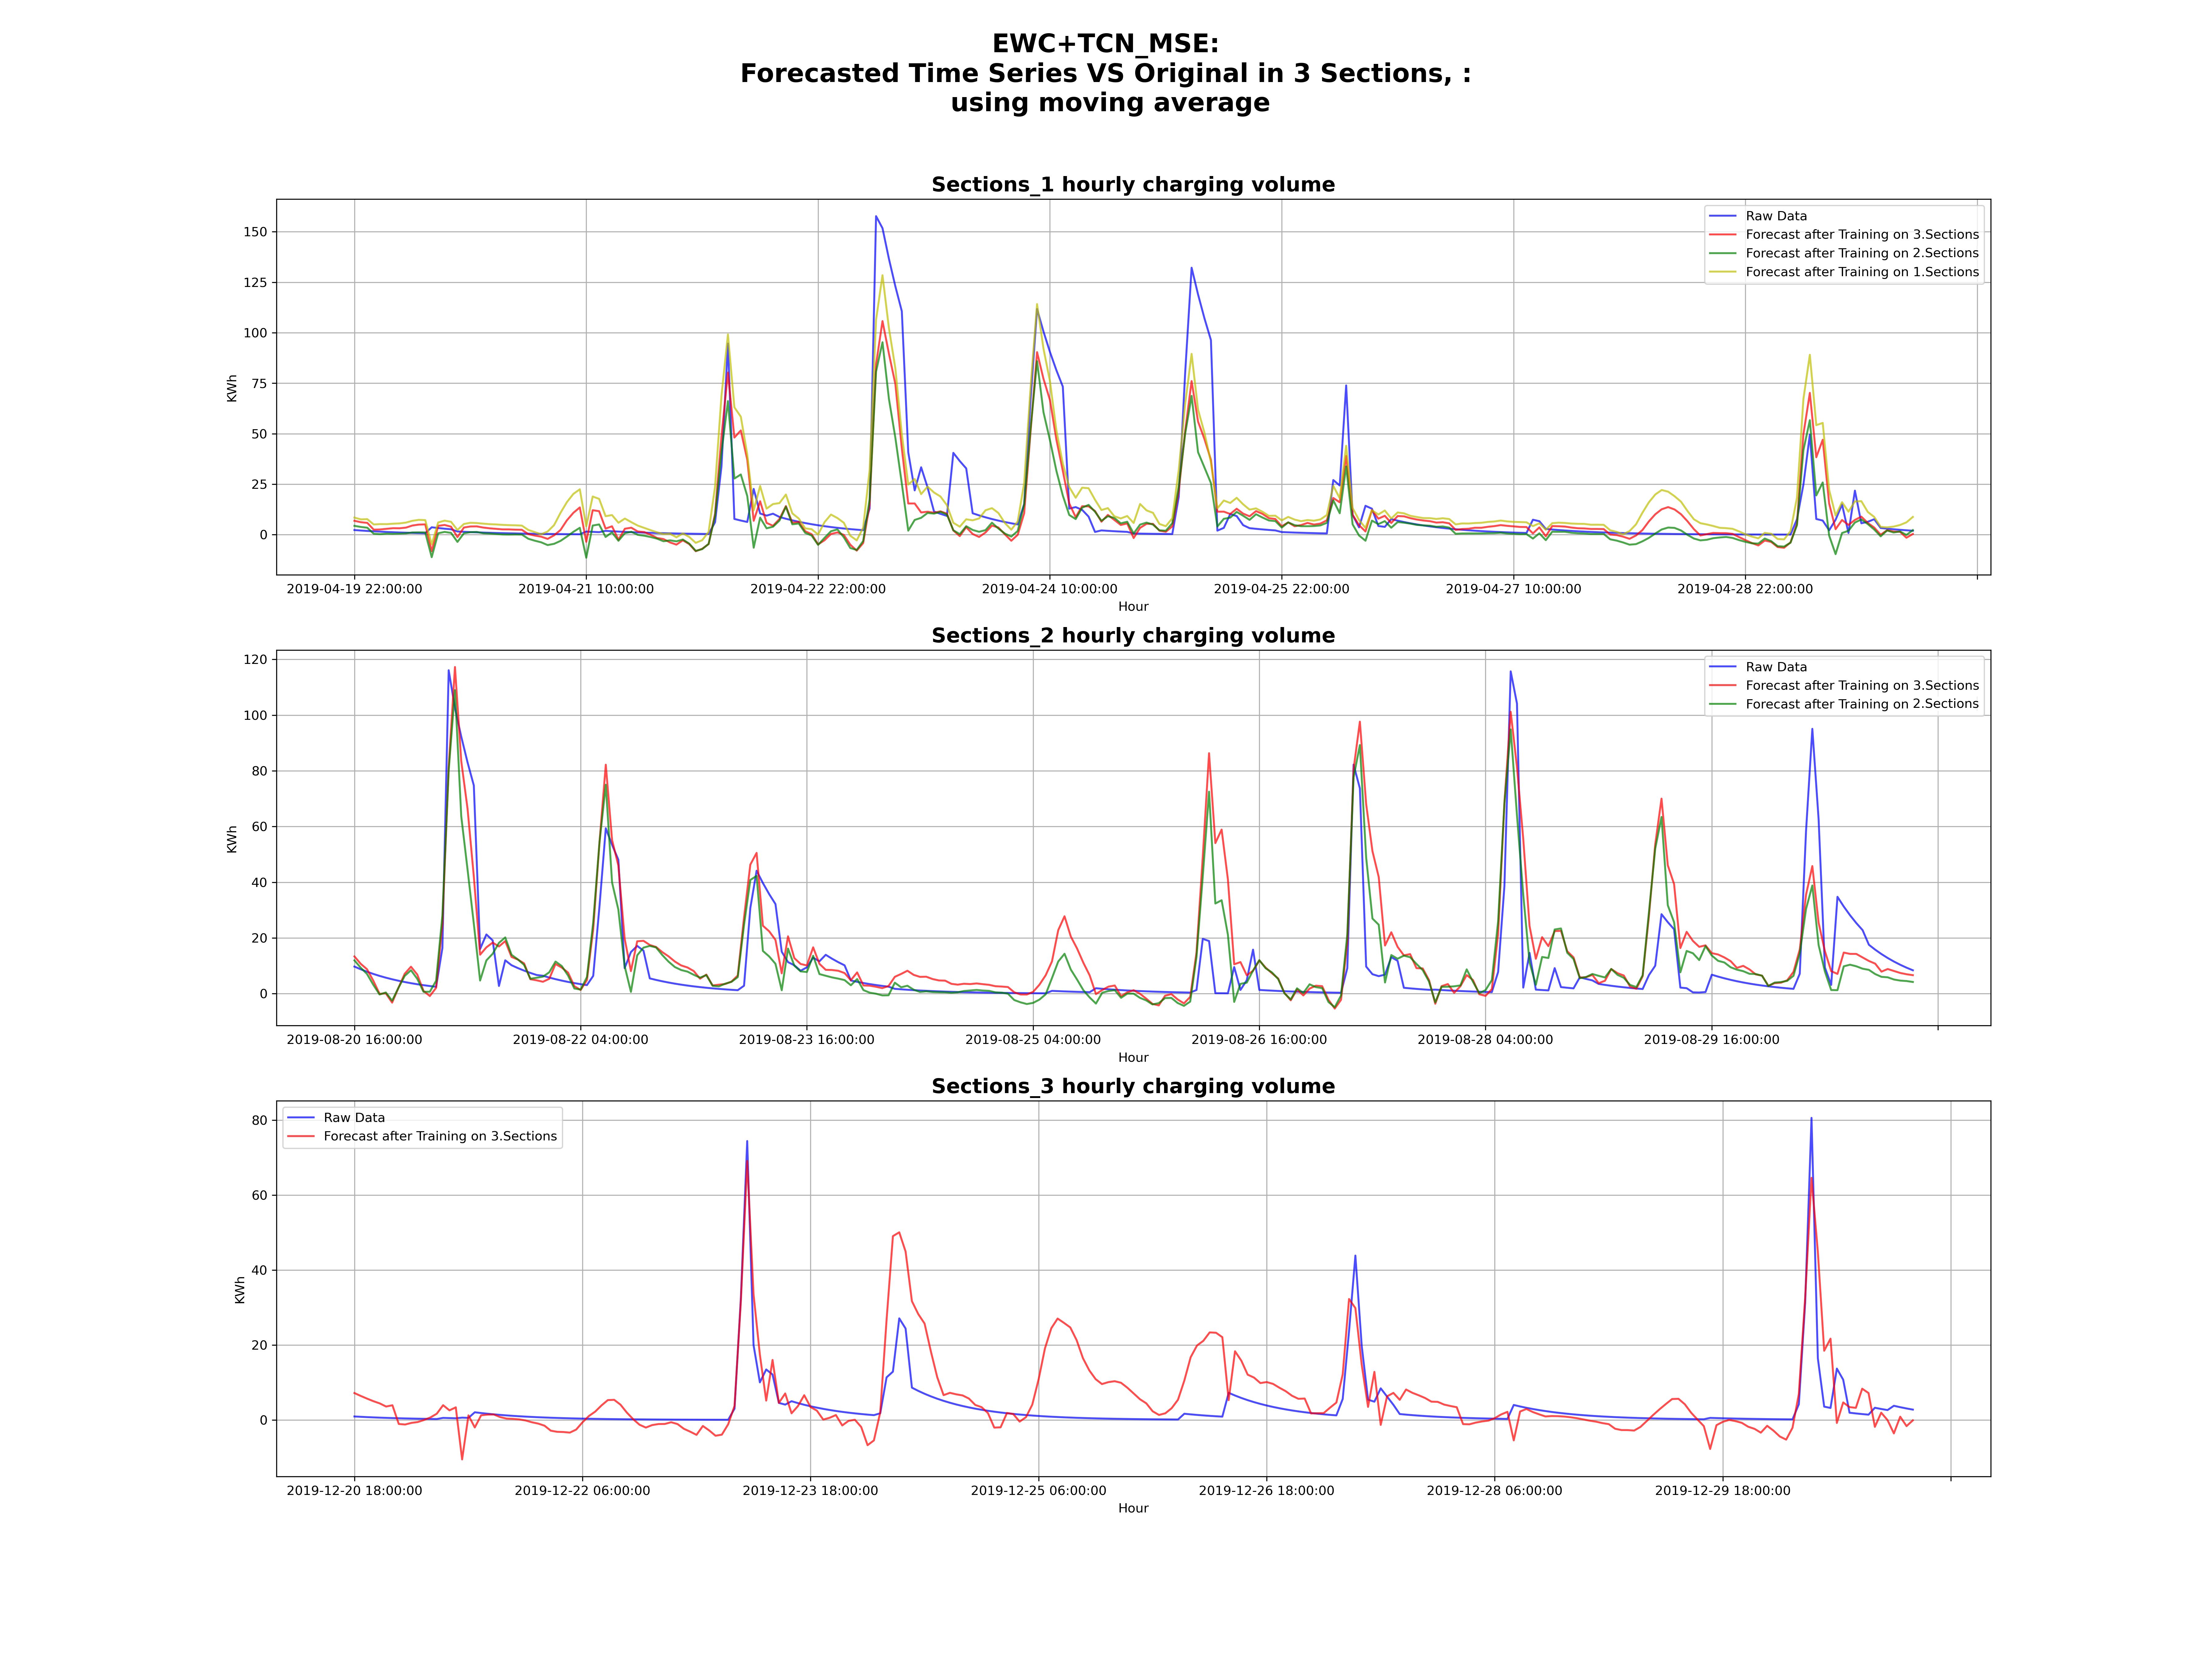
\includegraphics[width=.8\textwidth]{images/synthetic_forecast.png}
    \caption{CL experiment for synthetic data jpl site samples (created by Yuan Wang).}
    \label{fig:synth forecast}
\end{figure}
\chapter{Application}
\label{sec:application}
\section{Anonymization}
\label{sec:anonym}
An application that can be derived from our experiments, especially the openmeter experiments described in sections \ref{subsec:openemter} and \ref{subsec:OM res}, is anonymization. The openmeter dataset contains one categorical feature for each sensor - the sensor ID. This ID is already an unspecific unique ID but can still point to a specific sensor located in a specific household. Through the experiments, it was shown that this ID is not important for the task of generating synthetic data. Authentic samples can be generated using more general features during training/sampling.

It has been demonstrated that the same principle would likely apply to the LSM experiments, which completely rely on unique IDs since there were no other features to work with.
Training models and then performing state 
estimations or different forecasting tasks and publishing these models to the public seems to evade the problems that might arise with privacy issues. Openmeter itself solves this problem by giving the people the opportunity to upload their data by themselves so they give personal consent. 
Future energy supplier might consider opening their data to science, energy applications or the public in general by providing a well trained generative model.

\section{State estimations and other simulations}
\label{sec:state estem}
During this thesis some of the generated data were used in experiments. Those experiments and evaluations are at the moment of this thesis still ongoing so there is no way of refer to actual results but there is applicable value that will be addressed. This goes not only hand in hand with the anonymization described in the section above but also takes scientific value into account. Generative models can be used to have an easily callable generator that supplies different kinds of complex simulations with the necessary input data. In this case electrical network state estimator were supplied with generated data. Exemplary this data was used to prototype certain situations that couldn't be easily or cheaply recreated with real world data. The model gave a flexible alternative.

\section{Continual learning support models}
\label{sec:apply cl}
One of the mayor research questions that concerns various data scientist and will be discussed in this thesis is the question of continual learning. During the evaluation phase of the ACN data samples described in \ref{subsec:ACN res}  an introduction of a continual learning setup as a applicative test was made. In this case, the models were used as CL tools, but the presented generated models themselves could be  embedded in continual learning scenarios to further improve the result of those test. Such approaches can be found in \cite{shin2017continual}. In the future this can be seen as method to save time and resources since it is not necessary to rely on an entire dataset but rather a generator structure that compressed the information of such dataset.
\chapter{Conclusion}
\label{sec:conclusion}
With the proposed methods described in chapter \ref{sec:approach}, authentic samples that resemble the dataset described in chapter \ref{sec:datasets} were successfully generated.
This task was achieved by a DDPM model that is capable of generating time series data. 
By restructuring the UNET to 1-dimensional convolution model, the overall DDPM was able to learn the denoising process described in \ref{sec:ddpm}. Generating time series samples is now possible.
The quality of those generated samples is undermined by the decent scoring in chapter \ref{sec:results}. 
The different described metrics and statistical evaluation methods suggest a good synthetic representation of the initial dataset. 
So for the question of whether DDPM are capable for time series synthesis it is conclude that the assumptions were met positively, but still can be improved through extensive hyper parameter optimization or switching to an other model architecture besides UNET.
Going into the next phase of applicative testing, described in chapter \ref{sec:experiments}, the top performing models where plugged into the described continual learning scenario.
Supplying the forecasting model with synthetic samples to test the training process through different stages of the experiences defined in the 
scenario resulted in an overall similar training performance. The accuracy of the forecasting model was slightly worse during the varying tasks. So our synthetic samples also performed almost identical to real data which is a hint for good quality in a practical setting. Not only is it another indicator for a successfully time series DDPM but also 
can verify the assumption that DDPMs can perform continual learning environment. The overall conclusion is that all assumptions were satisfied.
\section*{Outlook}
Future research topics that are interesting could be more appliance test on other tasks that benefit from synthetic time series samples. 
Also the question of anonymization of sensible time series data in the public or health care sector are fascinating venues that can be explored. And the results in this thesis can be put onto testing in other fields that differ from EV or household power consumption. Since the topic of time series data is a broad plane of potentials the presented approaches and models could be tested for different scenarios in various fields of research. Since the first release of image generation models further improvements were made to them. It is possible to perform different style transfers, upscale images, inpaint or change parts in an image or transform it into another genre keeping the underlying information. Those augmentations should also be possible for the domain of time series data and might present a vault of interesting research questions.\newline
The idea of implementing generative models into continual learning setup was already roughly sketched in section \ref{sec:apply cl}. Using generative models as support models in different CL scenarios may boost the overall CL performance. Retaining previous tasks by supplying compact models instead of entire datasets might be the solution for efficient and sustainable model training in the future. In this case we see generative models as a tool to enhance CL tasks. But it was also imminent that generative models could be seen as the target for CL research. The models are currently trained on temporal data. The overall behavior might change for the coming years, which means that the generative models are getting worse and worse representatives for the real world. So continually improving the models and still retaining the old information is also for generative models an important problem that needs to be investigated.
\cleardoublepage
\pagenumbering{roman}
\appendix
\chapter{Appendix}
\captionsetup{list=no}
\begin{table}[h!]
    \centering
    \begin{tabular}{|c c | c c | c c|} 
        \multicolumn{6}{c}{univariate mmd scores}\\
        \hline
        batch & mmd score & batch & mmd score  & batch & mmd score \\
        \hline\hline
        lsm 01 & 0.001095 &
        lsm 02 & 0.001189 &
        lsm 03 & 0.000248 \\
        lsm 04 & 0.004695 &
        lsm 05 & 0.000790 &
        lsm 06 & 0.022553 \\
        lsm 07 & 0.006913 &
        lsm 08 & \textbf{\textcolor{blue}{0.000203}} &
        lsm 09 & 0.003571 \\
        lsm 10 & 0.001193 &
        lsm 11 & 0.000987 &
        lsm 12 & 0.002153 \\
        lsm 13 & 0.001272 &
        lsm 14 & 0.000353 &
        lsm 15 & 0.000683 \\
        lsm 16 & 0.000852 &
        lsm 17 & 0.001853 &
        lsm 18 & 0.000379 \\
        lsm 19 & 0.004669 &
        lsm 20 & 0.001623 &
        lsm 21 & 0.001134 \\
        lsm 22 & 0.003864 &
        lsm 23 & 0.001535 &
        lsm 24 & 0.001667 \\
        lsm 25 & 0.004149 &
        lsm 26 & 0.010215 &
        lsm 27 & 0.007429 \\
        lsm 28 & 0.000372 &
        lsm 29 & 0.006910 &
        lsm 30 & 0.002412 \\
        lsm 31 & 0.003552 &
        lsm 32 & 0.000283 &
        lsm 33 & 0.006011 \\
        lsm 34 & 0.005022 &
        lsm 35 & 0.000650 &
        lsm 36 & 0.001387 \\
        lsm 37 & 0.005250 &
        lsm 38 & 0.004809 &
        lsm 39 & 0.006311 \\
        lsm 40 & 0.001373 &
        lsm 41 & 0.000411 &
        lsm 42 & 0.000560 \\
        lsm 43 & \textbf{\textcolor{red}{0.030736}} &
        lsm 44 & 0.000643 &
        lsm 45 & 0.001401 \\
        lsm 46 & 0.004326 &
        lsm 47 & 0.002762 &
        lsm 48 & 0.000899 \\
        lsm 49 & 0.002654 &
        lsm 50 & 0.002061 &
        lsm 51 & 0.001648 \\
        lsm 52 & 0.006343 &
        lsm 53 & 0.002718 &
        lsm 54 & 0.003370 \\
        \hline
        \multicolumn{6}{c}{mean: 0.003569}
    \end{tabular}

    \begin{tabular}{|c c |c c| c c|}
        \multicolumn{6}{c}{multivariate mmd scores}\\
        \hline
        batch & mmd score & batch & mmd score & batch & mmd score\\
        \hline\hline
        lsm 01 & 0.004302 &
        lsm 02 & 0.001880 &
        lsm 03 & 0.001095 \\
        lsm 04 & 0.002974 &
        lsm 05 & 0.005337 &
        lsm 06 & 0.006210 \\
        lsm 07 & 0.004319 &
        lsm 08 & 0.005429 &
        lsm 09 & 0.007599 \\
        lsm 10 & 0.001365 &
        lsm 11 & 0.002206 &
        lsm 12 & 0.004846 \\
        lsm 13 & 0.002317 &
        lsm 14 & 0.002696 &
        lsm 15 & 0.001315 \\
        lsm 16 & 0.000821 &
        lsm 17 & 0.012402 &
        lsm 18 & 0.008775 \\
        lsm 19 & 0.014695 &
        lsm 20 & 0.002632 &
        lsm 21 & 0.003236 \\
        lsm 22 & 0.001471 &
        lsm 23 & 0.005080 &
        lsm 24 & 0.006379 \\
        lsm 25 & 0.001095 &
        lsm 26 & 0.003414 &
        lsm 27 & 0.011945 \\
        lsm 28 & 0.002359 &
        lsm 29 & 0.003644 &
        lsm 30 & 0.007566 \\
        lsm 31 & 0.007163 &
        lsm 32 & \textbf{\textcolor{red}{0.036864}}&
        lsm 33 & 0.007520 \\
        lsm 34 & 0.006216 &
        lsm 35 & 0.008992 &
        lsm 36 & 0.004288 \\
        lsm 37 & 0.002008 &
        lsm 38 & 0.011144 &
        lsm 39 & 0.004037 \\
        lsm 40 & 0.001489 &
        lsm 41 & 0.002060 &
        lsm 42 & 0.013073 \\
        lsm 43 & 0.009164 &
        lsm 44 & 0.001884 &
        lsm 45 & 0.001099 \\
        lsm 46 & 0.002816 &
        lsm 47 & 0.011187 &
        lsm 48 & 0.001550 \\
        lsm 49 & 0.001935 &
        lsm 50 & 0.001988 &
        lsm 51 & 0.006244 \\
        lsm 52 & 0.005689 &
        lsm 53 & 0.004562 &
        lsm 54 & \textbf{\textcolor{blue}{0.000449}}\\
        \hline
        \multicolumn{6}{c}{mean: 0.005349}
    \end{tabular}
    \caption{All mmd score results for univariate and multivariate LSM models.}
    \label{table:lsm results}
\end{table}
\begin{figure}
    \centering
    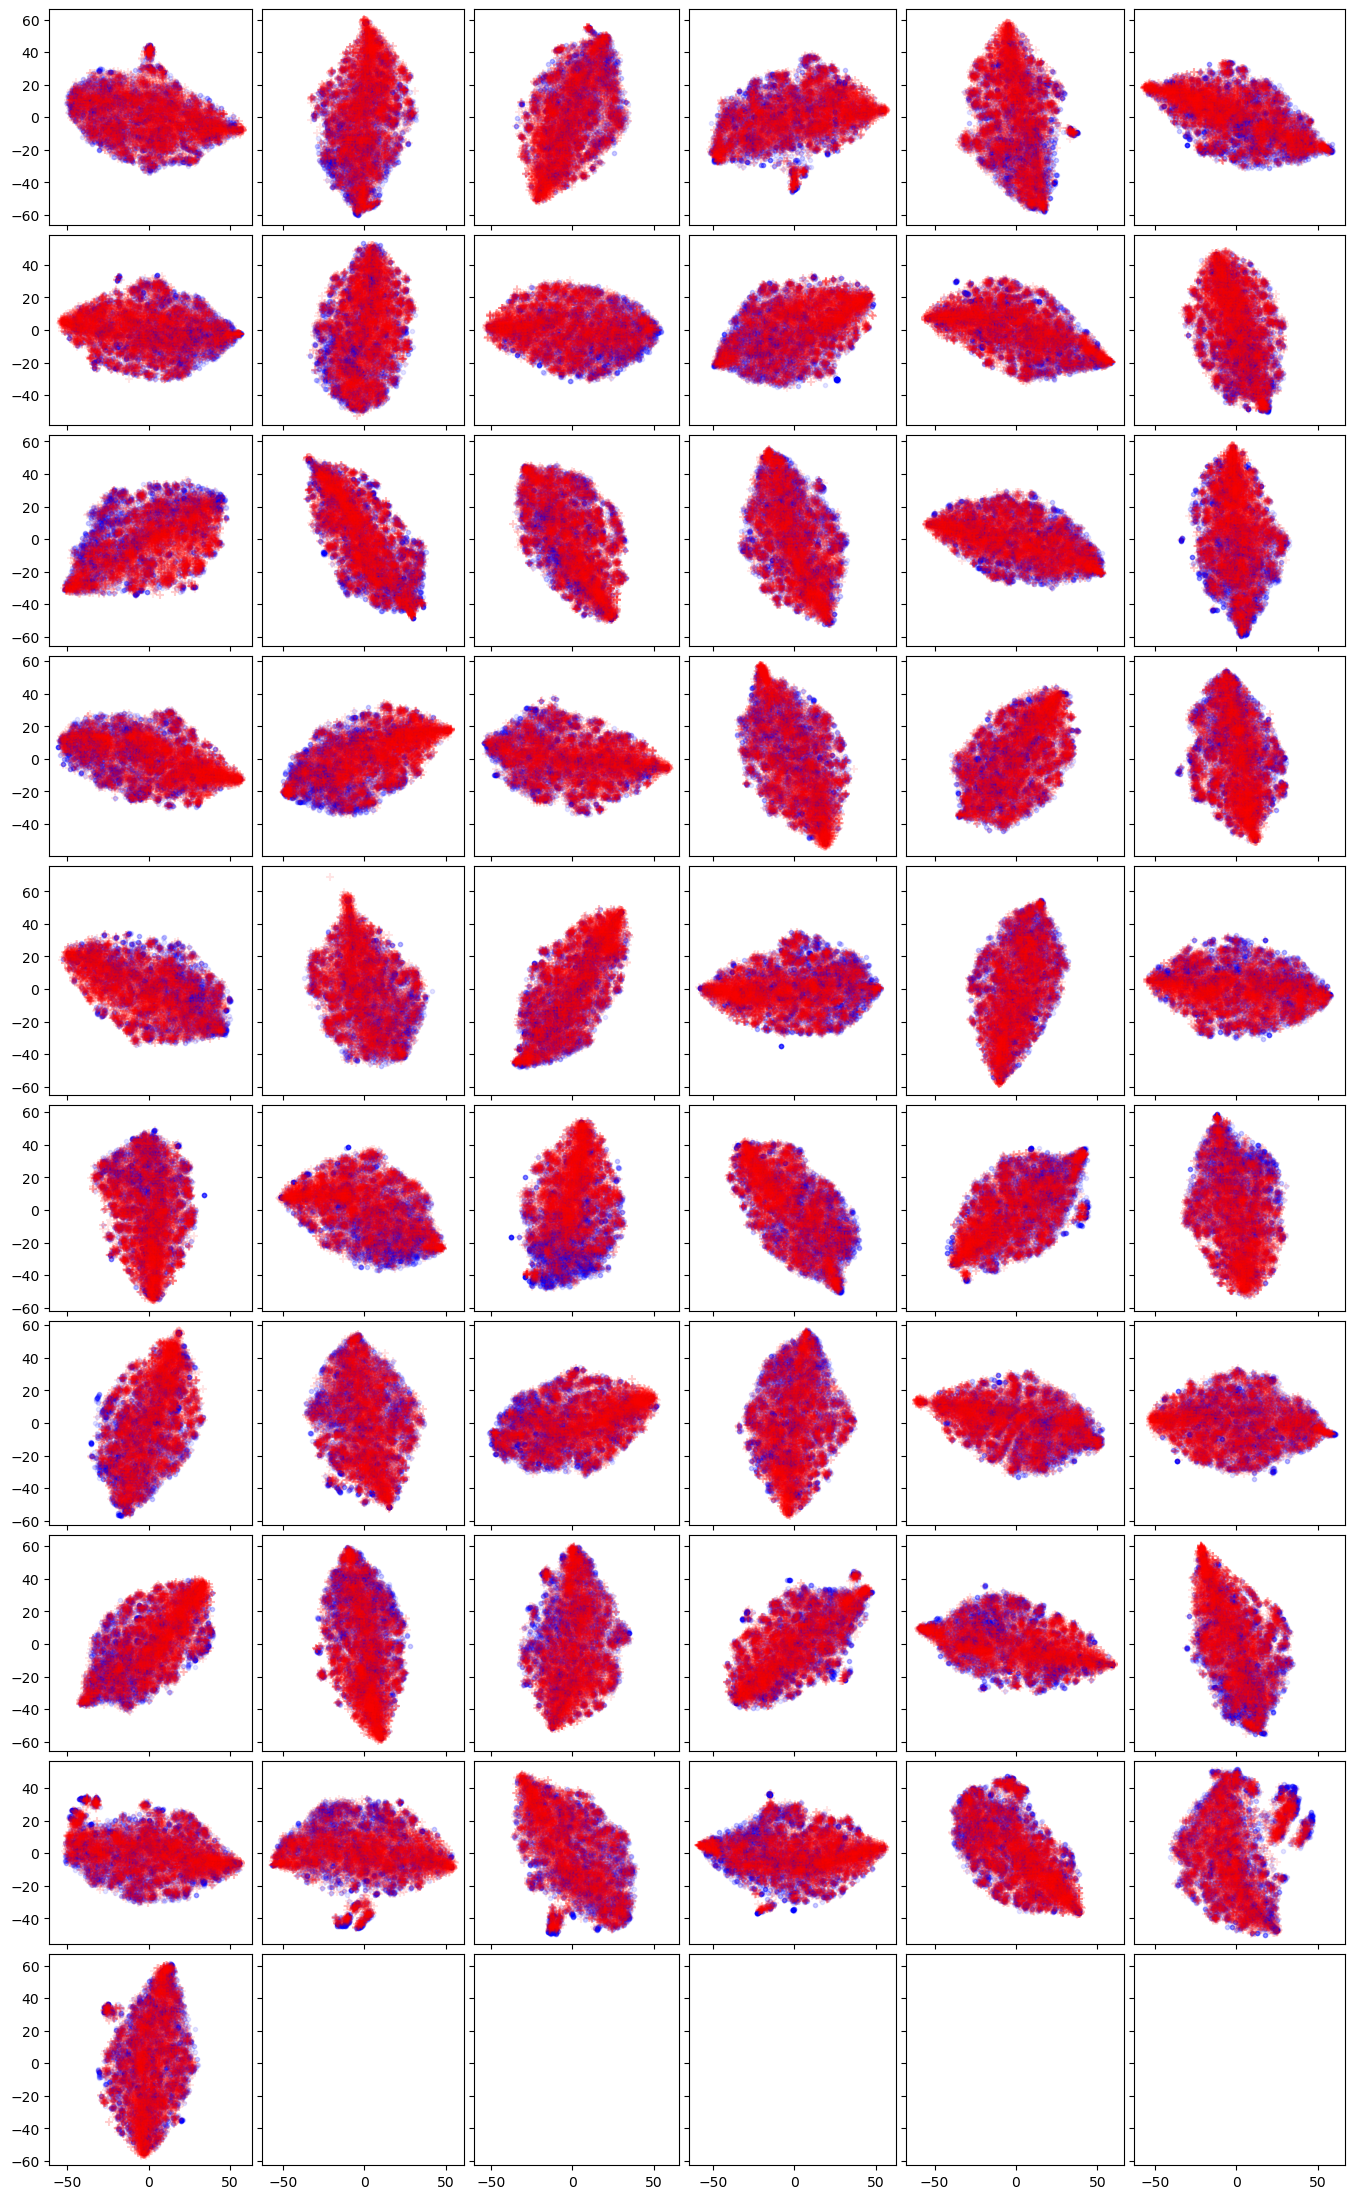
\includegraphics[height=\textheight]{images/tsen_overall_mult.png}
    \caption{TSNE batch results for multivariate experiments.}
    \label{fig:tsne overall mult}
\end{figure}
\begin{figure}
    \centering
    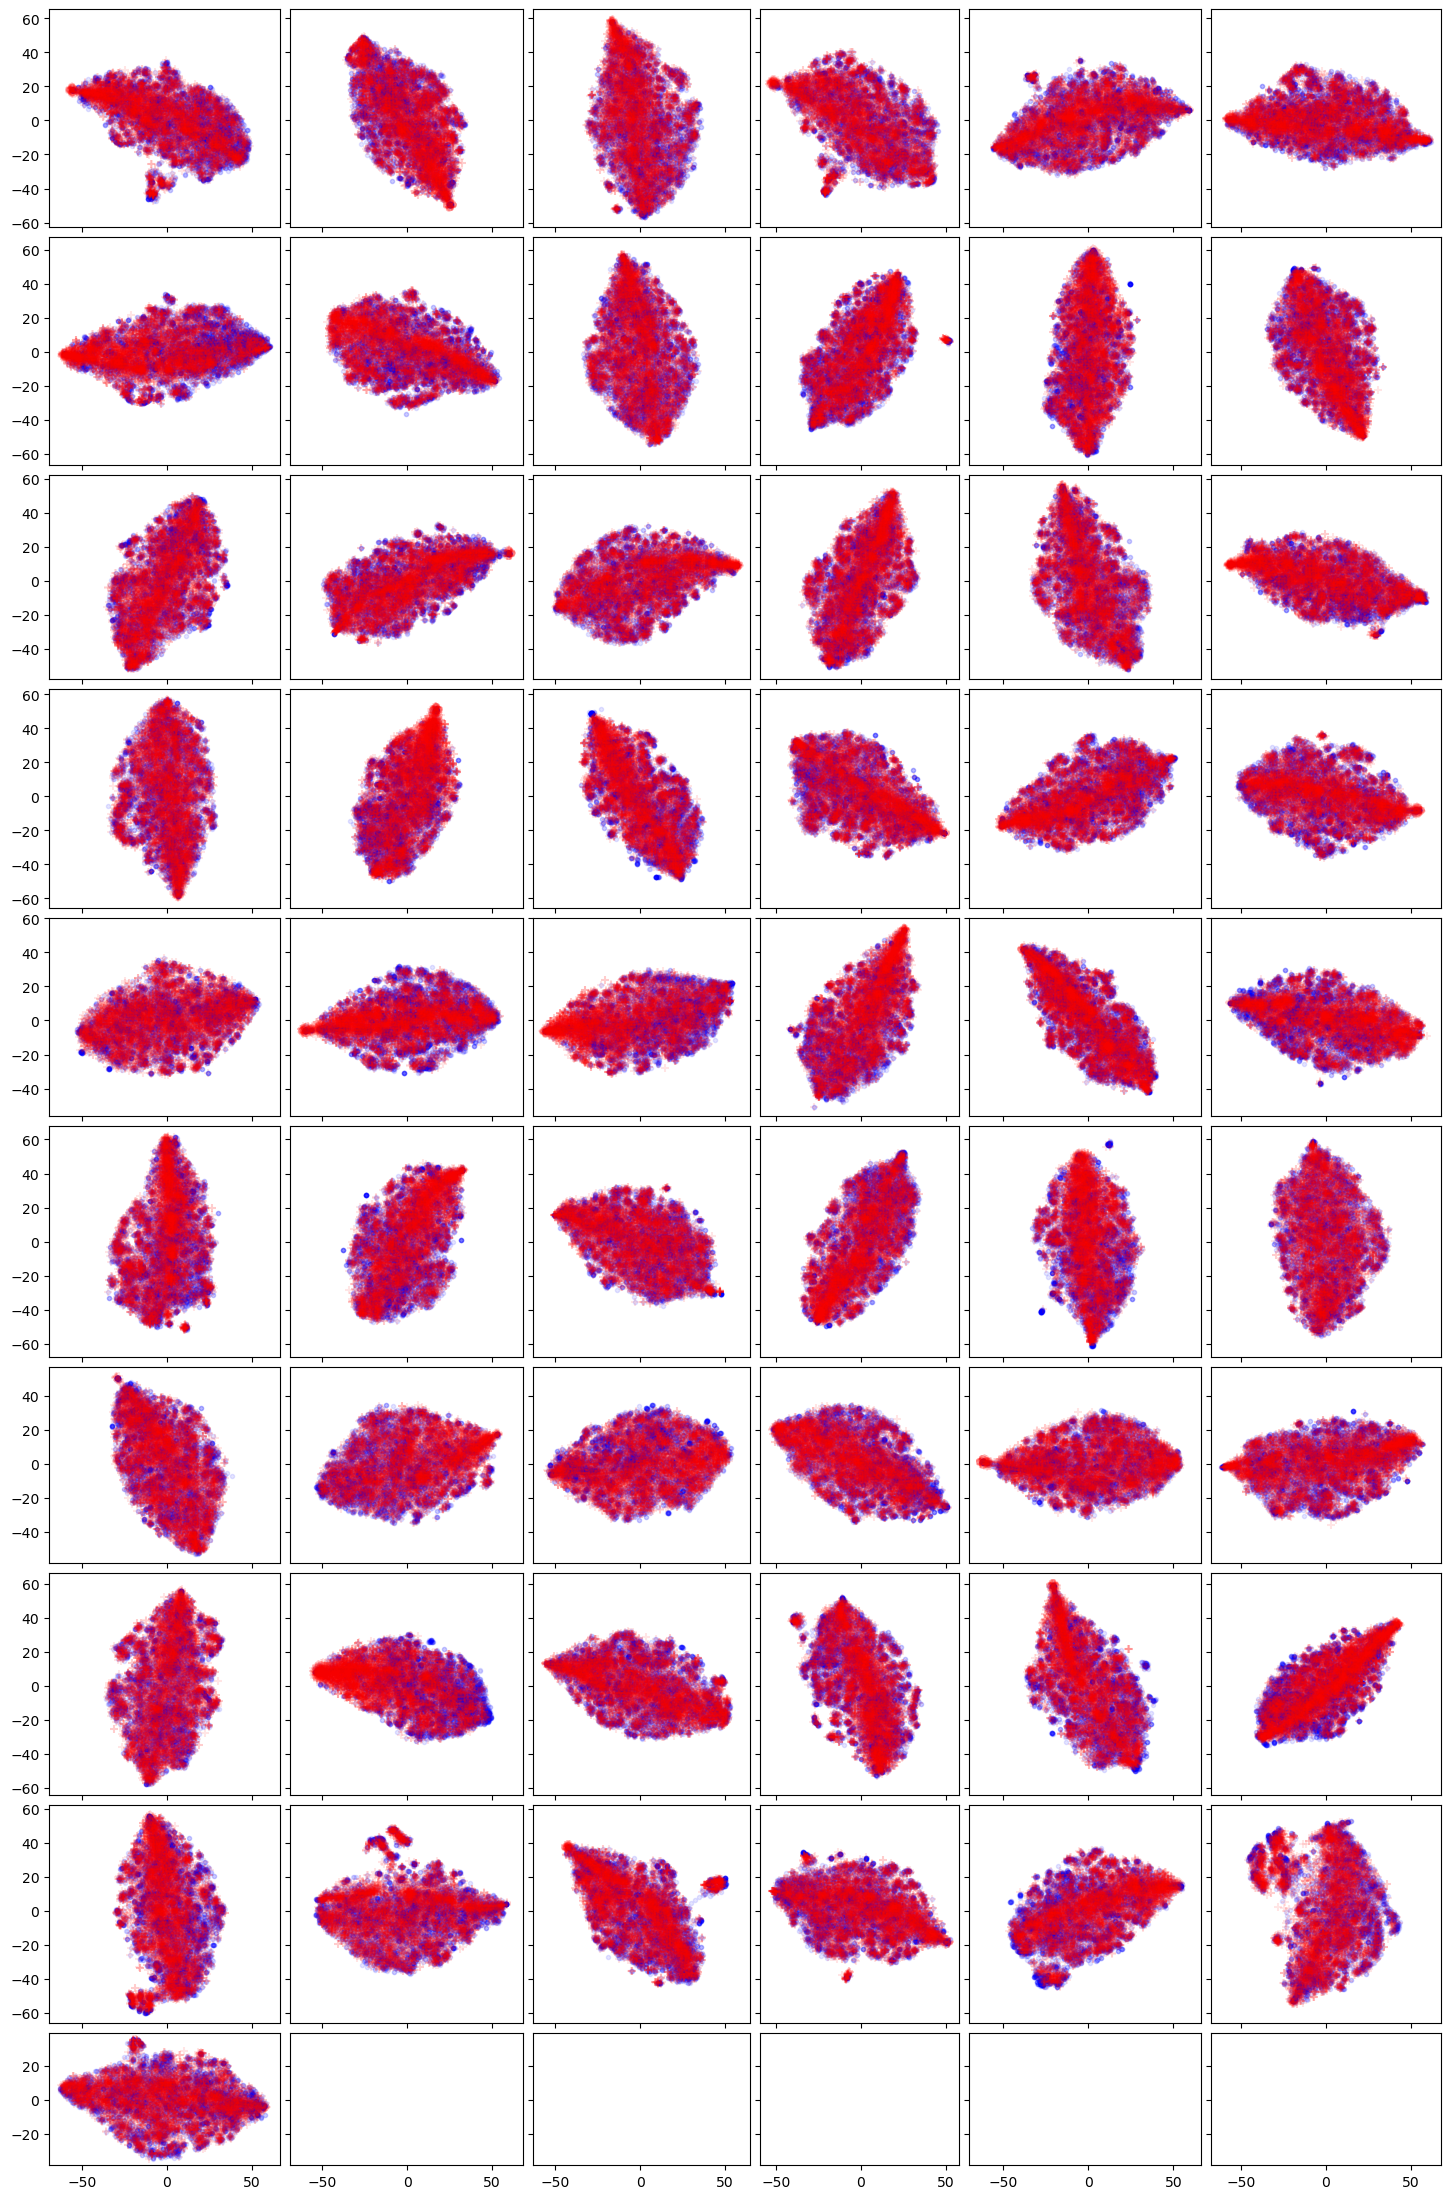
\includegraphics[height=\textheight]{images/tsen_overall_uni.png}
    \caption{TSNE batch results for univariate experiments.}
    \label{fig:tsne overall uni}
\end{figure}
\begin{figure}
    \centering
    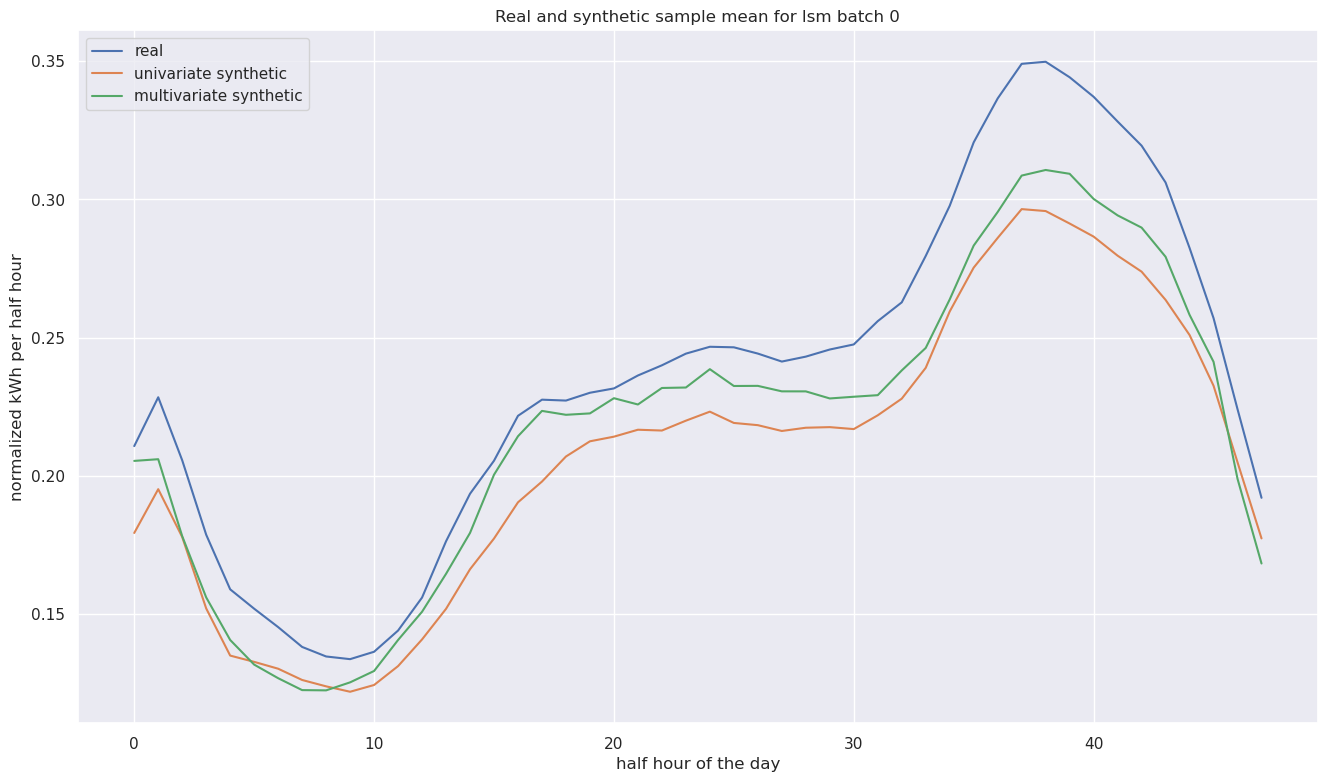
\includegraphics[width=\textwidth]{images/lsm_dm_0.png}
    \caption{Real and generated sample mean for lsm batch 0}
    \label{fig:sample mean 09}
\end{figure}
\begin{figure}
    \centering
    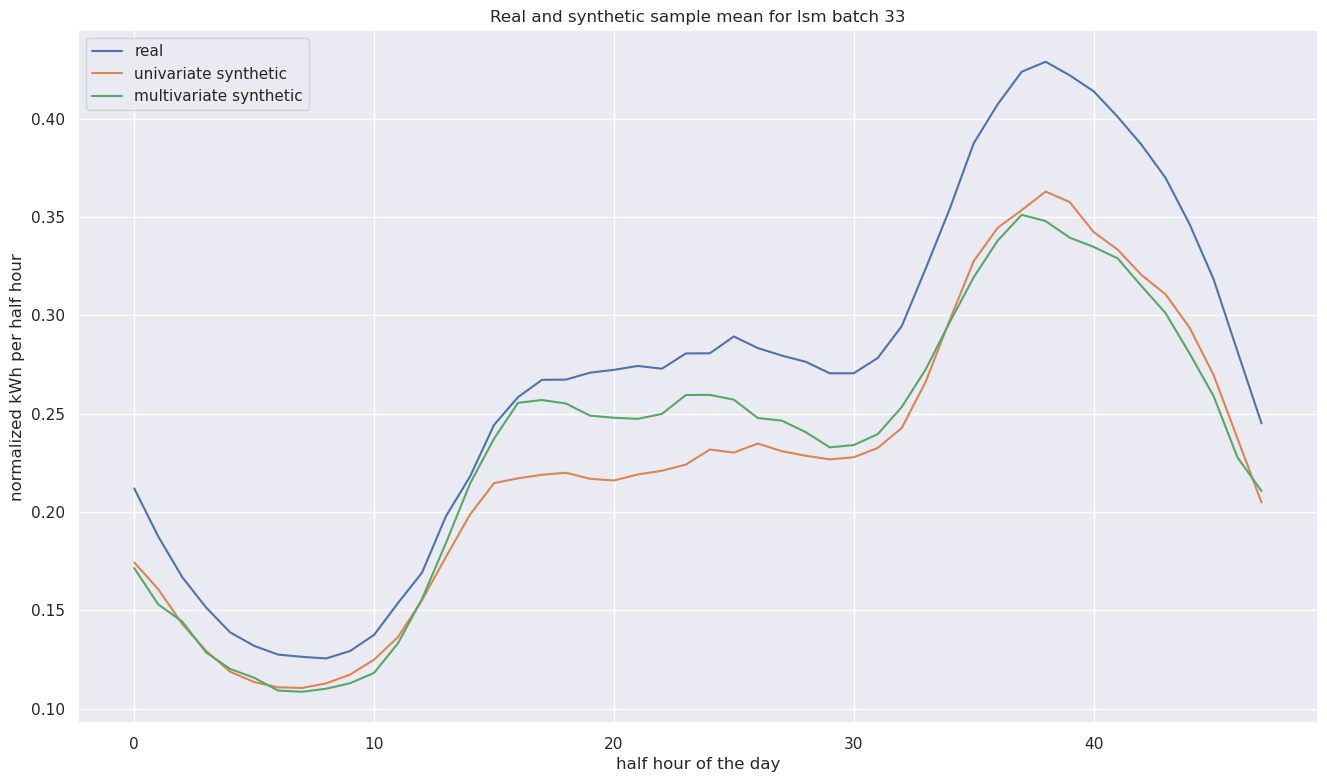
\includegraphics[width=\textwidth]{images/lsm_dm_33.png}
    \caption{Real and generated sample mean for lsm batch 33}
    \label{fig:sample mean 37}
\end{figure}
\begin{figure}
    \centering
    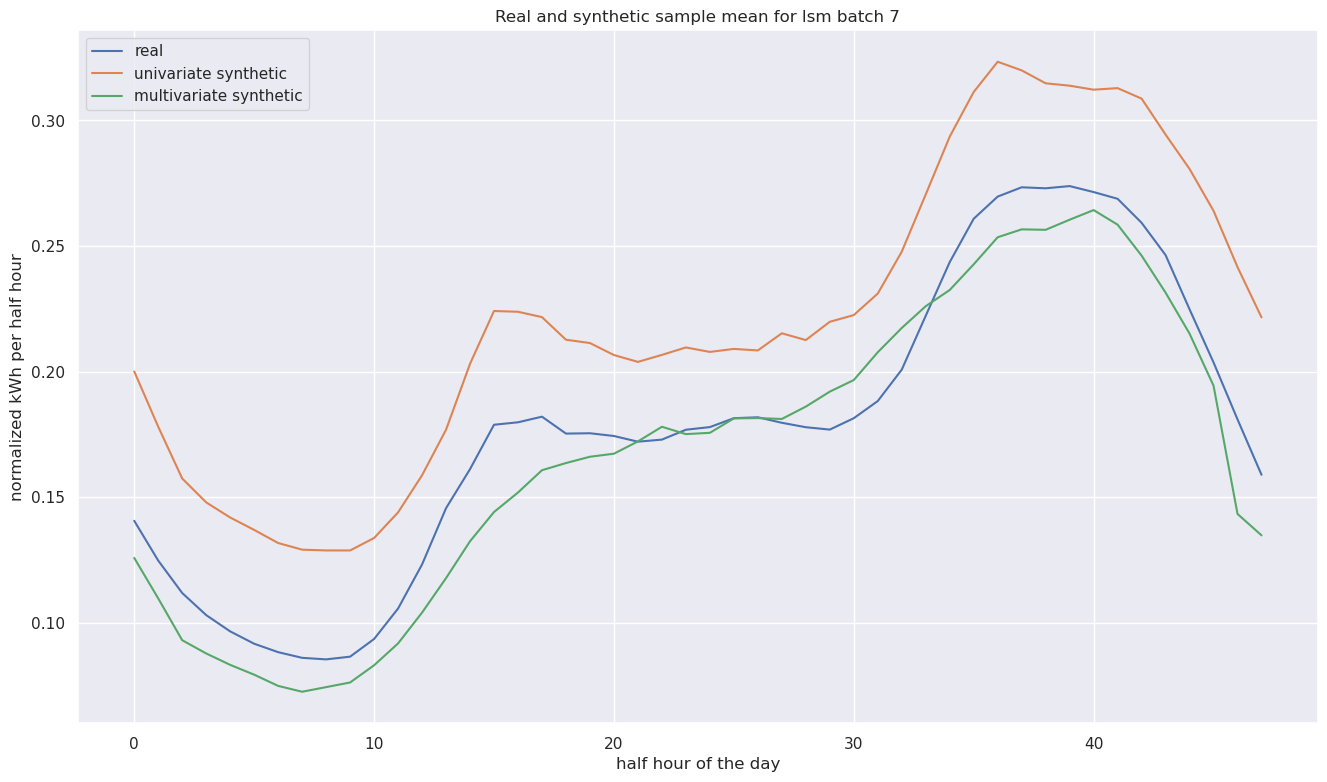
\includegraphics[width=\textwidth]{images/lsm_dm_7.png}
    \caption{Real and generated sample mean for lsm batch 7}
    \label{fig:sample mean 53}
\end{figure}
\begin{figure}
    \centering
    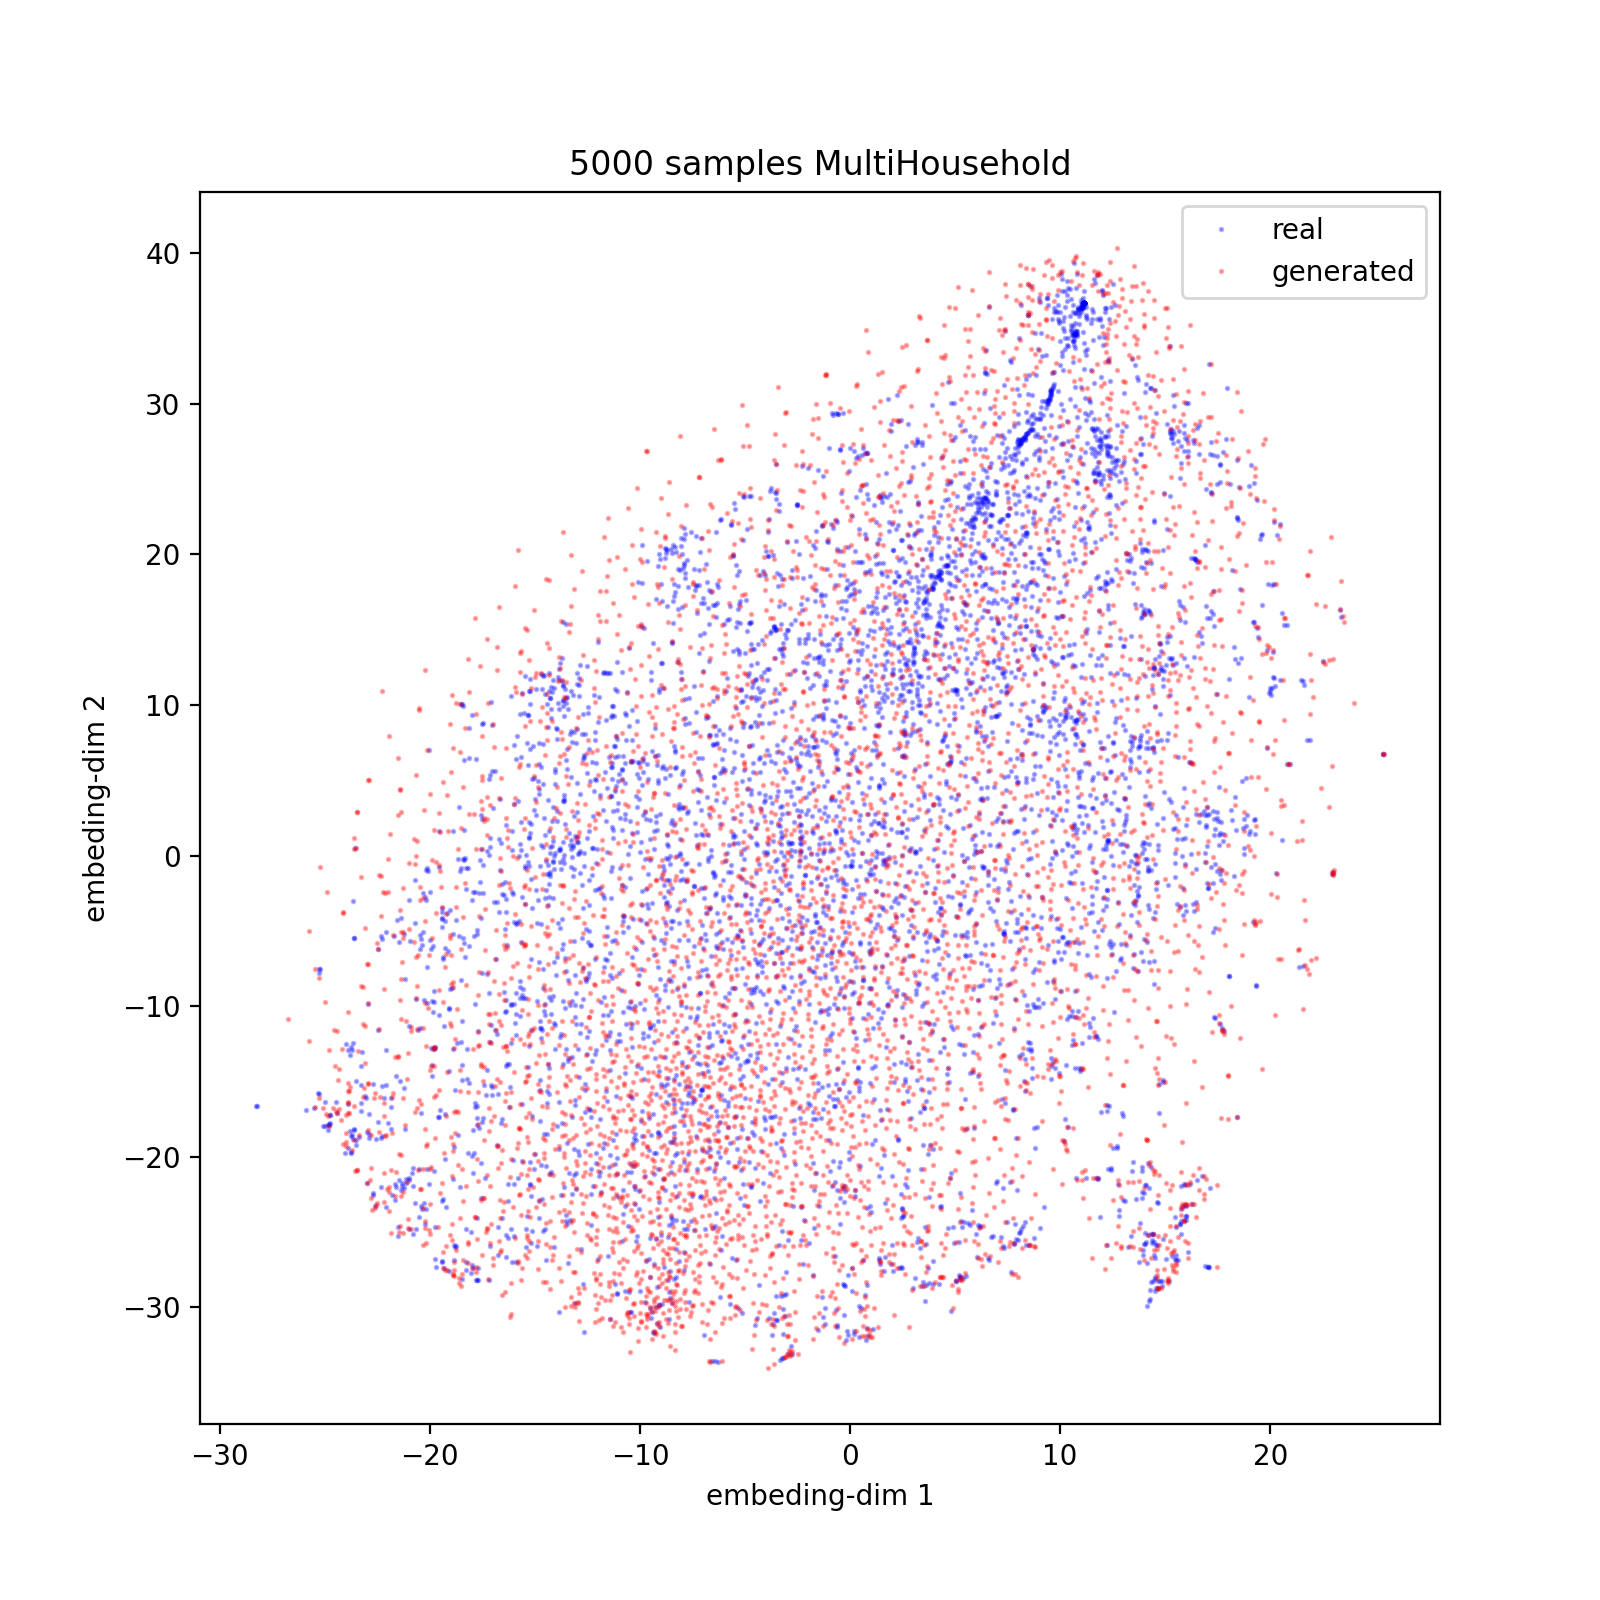
\includegraphics[width=0.85\textwidth]{images/om_uni_tsne.png}
    \caption{Univariate t-SNE samples from openmeter experiments.}
    \label{fig:om tsne uni}
\end{figure}
\begin{figure}
    \centering
    \begin{subfigure}[b]{0.45\textwidth}
        \centering
        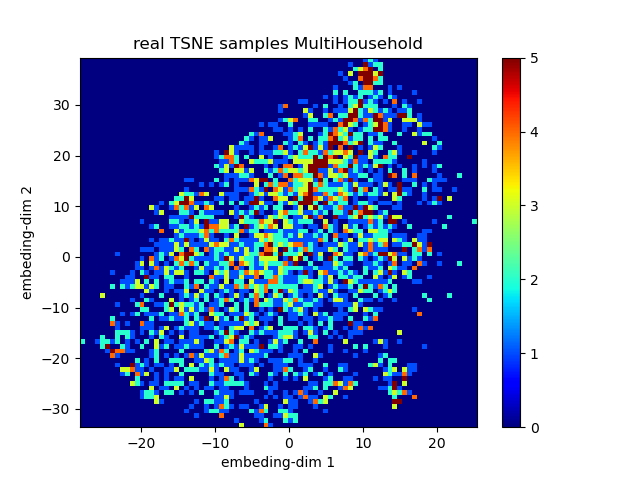
\includegraphics[width=\textwidth]{images/om_uni_real_histo.png}
        \caption{Univariate openmeter t-SNE histogram for real samples.}
        \label{fig:om tsne uni real histo}
    \end{subfigure}
    \begin{subfigure}[b]{0.45\textwidth}
        \centering
        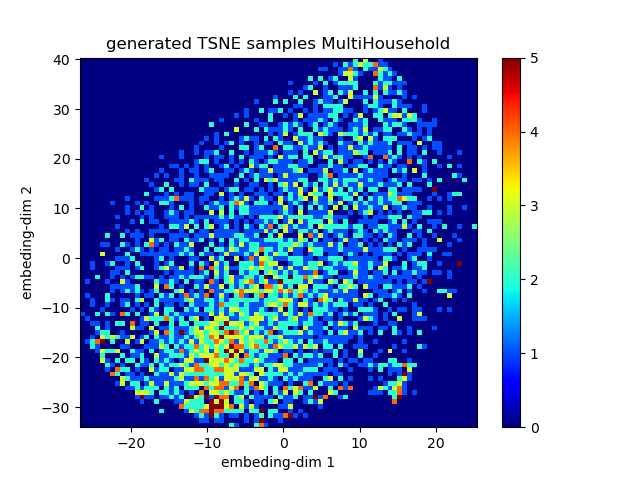
\includegraphics[width=\textwidth]{images/om_uni_fake_histo.png}
        \caption{Univariate openmeter t-SNE histogram for fake samples.}
        \label{fig:om tsne uni fake histo}
    \end{subfigure}
       \caption{Histogram of real and fake t-SNE samples for comparison.}
       \label{fig:om tsne uni histo}
\end{figure}

\begin{figure}
    \centering
    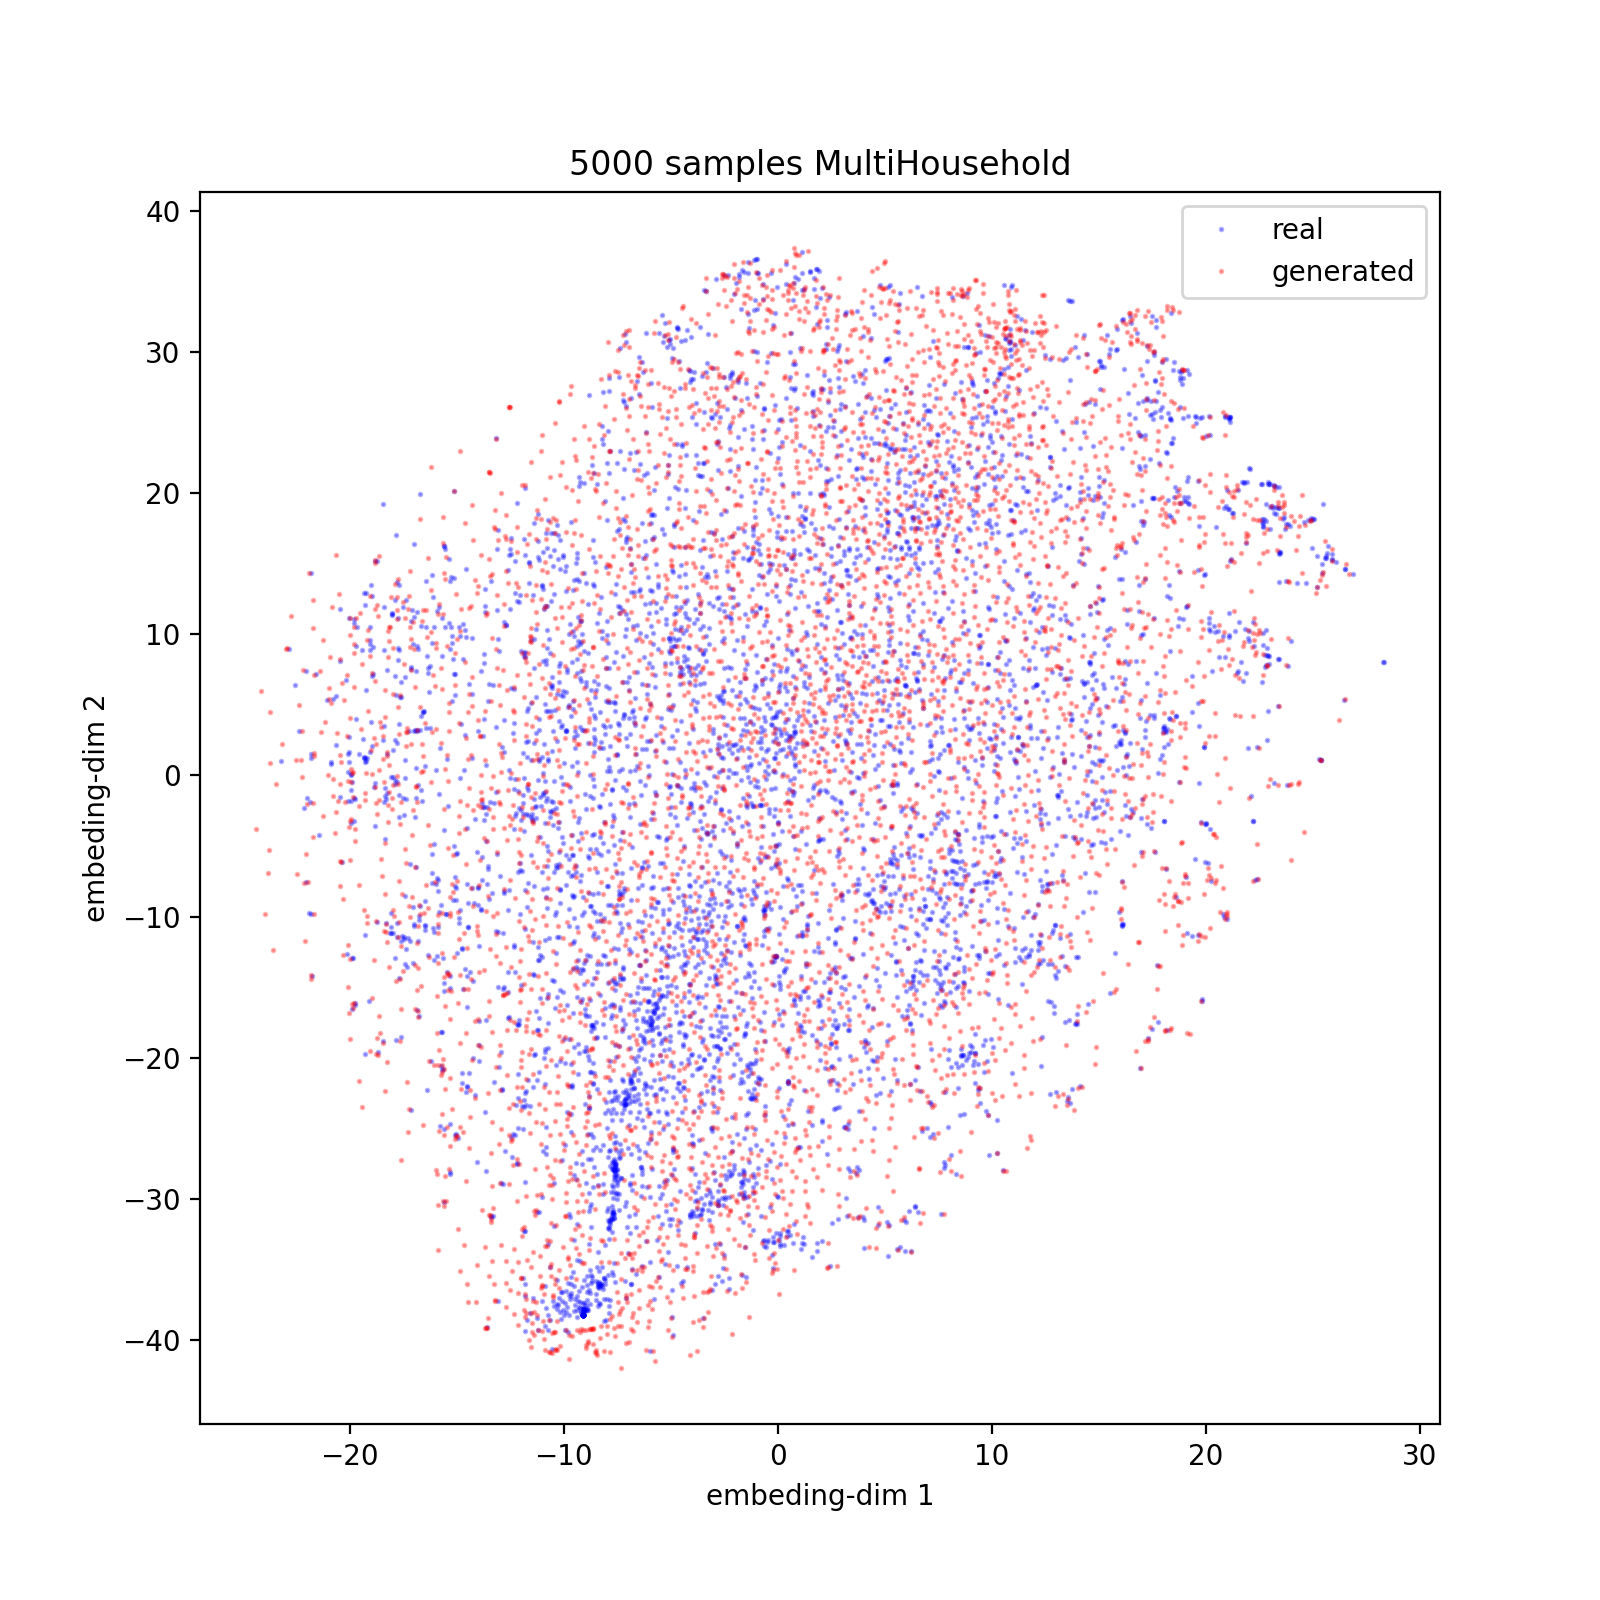
\includegraphics[width=0.85\textwidth]{images/om_multi_tsne.png}
    \caption{Multivariate t-SNE samples from openmeter experiments.}
    \label{fig:om tsne multi}
\end{figure}
\begin{figure}
    \centering
    \begin{subfigure}[b]{0.45\textwidth}
        \centering
        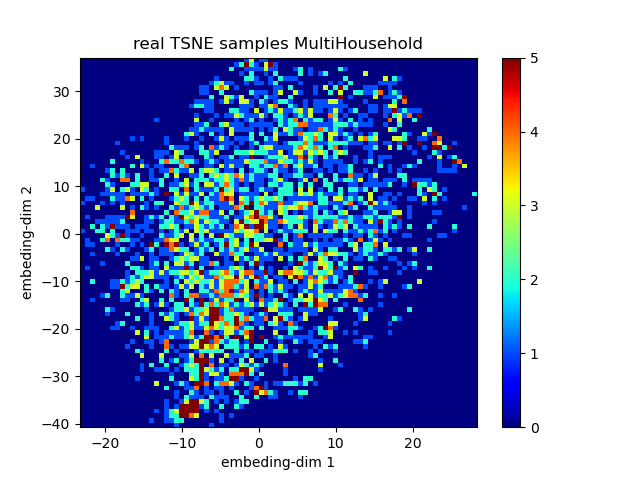
\includegraphics[width=\textwidth]{images/om_multi_real_histo.png}
        \caption{Multivariate openmeter t-SNE histogram for real samples.}
        \label{fig:om tsne multi real histo}
    \end{subfigure}
    \begin{subfigure}[b]{0.45\textwidth}
        \centering
        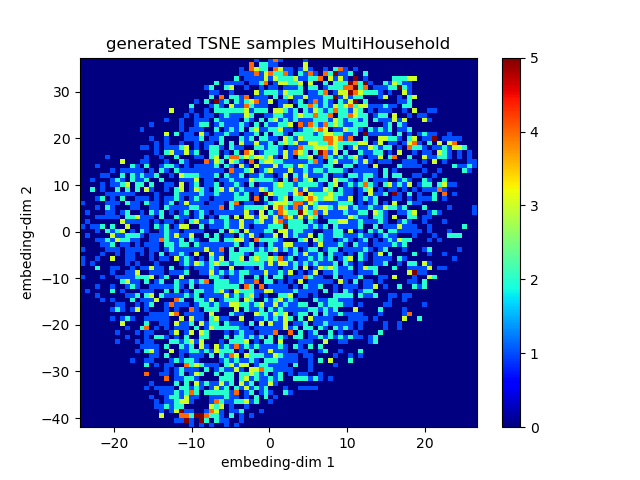
\includegraphics[width=\textwidth]{images/om_multi_fake_histo.png}
        \caption{Multivariate openmeter t-SNE histogram for fake samples.}
        \label{fig:om tsne multi fake histo}
    \end{subfigure}
       \caption{Histogram of real and fake t-SNE samples for comparison.}
       \label{fig:om tsne multi histo}
\end{figure}
\listoffigures
\listoftables
\newpage
%\bibliographystyle{apalike}
\bibliographystyle{alpha}
\bibliography{bib/references}
\chapter*{Eidesstattliche Erklärung}
%\addcontentsline{toc}{chapter}{Eidesstattliche Erklärung}

Ich erkläre hiermit an Eides statt, dass ich diese Diplomarbeit
mit dem Titel "Time Series Denoising Diffusion Probabilistic Models and Continual Learning" selbstständig und ohne Benutzung anderer als der angegebenen Quellen und Hilfsmittel angefertigt habe. Alle Ausführ\-ungen, die wörtlich oder sinngemäß übernommen wurden, habe ich als solche gekennzeichnet. Diese Diplomarbeit wurde in gleicher oder ähnlicher Form noch keiner anderen Prüfungsbehörde vorgelegt.\\
	\vspace{3em}
	\\
	Kassel, den \today \ \ \ \underline{\ \ \ \ \ \ \ \ \ \ \ \ \ \ \ \ \ \ \ \ \ \ \ \ \ \ \ \ \ \ \ \ \ \ \ \ \ \ }\\
	\hspace*{16.6em}\small{\ Unterschrift}
\end{document}

